\ExerciseGroupsStart
\ExerciseSection

\begin{enumerate}
\def\labelenumi{\arabic{enumi})}
\tightlist
\item
  * a) 设 \(f\) 是加法群 \(\mathbf{R}\) 到其自身的同态。证明：若 \(f\) 的图象在 \(\mathbf{R}^2\) 中不稠密，则 \(f\) 形如 \(x \to ax\) 。{[}考察 \(\mathbf{R}^2\) 中 \(f\) 的图象的闭包，并利用 \(\mathbf{R}^2\) 的闭子群结构定理（第 VII 章，§ 1，第 2 小节，定理 2）{]}。 * {[}试与第 VI 章，§ 1，习题 12 b) 以及第 IV 章，§ 6，习题 2 比较。{]}
\end{enumerate}

\begin{enumerate}
\def\labelenumi{\alph{enumi})}
\setcounter{enumi}{1}
\tightlist
\item
  若 f 的图象在 \(R^{2}\) 中稠密，则 \(R^{2}\) 的拓扑在映射 \(x \to (x, f(x))\) 下的逆像与 R 的群结构相容，且严格细于 R 的通常拓扑。若此外 f 还是单射，则 R 的通常拓扑在 f 下的逆像与 R 的群结构相容，且与 R 的通常拓扑不可比较。
\end{enumerate}

\begin{enumerate}
\def\labelenumi{\arabic{enumi})}
\setcounter{enumi}{1}
\tightlist
\item
  设 \(\mathfrak{C}\) 是 \(\mathbf{R}\) 上的豪斯多夫拓扑，它与 \(\mathbf{R}\) 的群结构相容，且严格粗于通常拓扑 \(\mathfrak{C}_0\) 。
\end{enumerate}

\begin{enumerate}
\def\labelenumi{\alph{enumi})}
\item
  证明：关于 \(\mathfrak{C}\)，o 的每个开邻域在 \(\mathbf{R}\) 中都无界（注意，粗于紧空间拓扑的豪斯多夫拓扑必与该拓扑一致）。
\item
  设 \(V \neq R\) 是关于 \(\mathfrak{C}\) 的 o 的一个对称开邻域，并设 W 是关于 \(\mathfrak{C}\) 的 o 的一个对称开邻域，满足 \(W + W \subset V\) 。证明：若 a 是 V 的包含 o 的那个连通分支（关于 \(\mathfrak{C}_{0}\)）的长度，则 W 的每个连通分支（关于 \(\mathfrak{C}_{0}\)）的长度都 \(\leqslant a\) 。此外，R - W 的内部（关于 \(\mathfrak{C}_{0}\)）的各连通分支的长度所成的集是有界的{[}利用 a) 以及存在 o 的对称开邻域 \(W_{1}\) （关于 \(\mathfrak{C}\)）使 \(W_{1} + W_{1} \subset W\) 这一事实{]}。
\item
  由 b) 推出：\(\mathbf{R}\) 在拓扑 \(\mathfrak{C}\) 下是预紧的且不是局部紧的。
\item
  同样证明：\(\mathbf{Z}\) 在任何与其群结构相容且异于离散拓扑的拓扑 \(\mathfrak{C}\) 下都是预紧的且不是局部紧的。
\item
  设 \(f\) 是 \(\Gamma\) （\(\mathbf{R}\) 的子群，不只由 o 组成，赋有由 \(\mathfrak{C}_0\) 诱导的拓扑）到完备豪斯多夫群 G 中的连续同态。证明：若 \(f\) 不是 \(\Gamma\) 到 \(f(\Gamma)\) （\(\mathbf{G}\) 的子群）上的同构，则 \(f(\Gamma)\) 在 \(\mathbf{G}\) 中是相对紧的{[}利用 \(c\) ) 与 \(d)\){]}。
\end{enumerate}

* \(f\) ) 对每个整数 \(n \geqslant 2\) ，给出连续单射同态 \(f\) （\(\mathbf{R}\) 到 \(\mathbf{T}^n\) 中的）的例子，使得 \(f(\mathbf{R})\) 在 \(\mathbf{T}^n\) 中稠密（参见第 VII 章，§ 1，第 4 小节，命题 7 的推论 1）。 *

\begin{enumerate}
\def\labelenumi{\arabic{enumi})}
\setcounter{enumi}{2}
\tightlist
\item
  证明群 \(\mathbf{T}\) 代数同构于乘积 \(\mathbf{R} \times (\mathbf{Q}/\mathbf{Z})\)（在 \(\mathbf{R}\) 中取一个适当的哈梅尔基）。由此推出：存在 \(\mathbf{R}\) 上的一个豪斯多夫拓扑，它与群结构相容，与通常拓扑不可比较，并且 \(\mathbf{R}\) 关于它是预紧的。
\end{enumerate}

\ExerciseSection

\begin{enumerate}
\def\labelenumi{\arabic{enumi})}
\tightlist
\item
  设 E 是具有最小元素 \(\omega\) 的全序集，并设 I 是 E 的一个区间，它包含 \(\omega\) ，并以 \(\omega\) 为其左端点。假设 E 与 I 满足公理 \((\mathrm{GR}_{\mathrm{I}}), (\mathrm{GR}_{\mathrm{II}}), (\mathrm{GR}_{\mathrm{IV}})\) 以及下面的公理：
\end{enumerate}

\((\mathrm{GR}_{\mathrm{III}b})\) I 中由元素 \(x > \omega\) 组成的集非空，且若 \(x\) 是 I 中任一 \(> \omega\) 的元素，则存在 I 中的 \(y > \omega\) 使得 \(y^2 \leqslant x\) 。

证明：存在递增映射 \(f\) （\(I\) 到 \(\mathbf{R}\) 中的），使得 \(f(\omega) = 0\) ，并且 \(f(xy) = f(x) + f(y)\) ，只要 \(x, y\) 与 \(xy\) 都属于 \(I\) ；并且 \(f(I) \cap [0, f(b)]\) 在 \([0, f(b)]\) 中稠密，对一切 \(b \in I\) 。

\begin{enumerate}
\def\labelenumi{\arabic{enumi})}
\setcounter{enumi}{1}
\tightlist
\item
  设 G 是非交换的全序群（例如非交换全序除环的乘法群）。在集合 \(R_{+} \times G\) 中考虑由 \((0, e)\)（e 为 G 的单位元）与所有偶 \((x, y)\)（其中 x 是任一实数 \textgreater0 ，而 y 是 G 的任一元素）所组成的集 E。用规则 \((x, y)(x', y') = (x + x', yy')\) 在 E 上定义一个合成律，并按字典序给 E 排序{[}即 \((x, y) < (x', y')\) 意为 \(x < x'\) ，或者 \(x = x'\) 且 \(y < y']\) 。若取 I = E，证明公理 \((\mathrm{GR}_{\mathbf{I}}), (\mathrm{GR}_{\mathbf{II}}), (\mathrm{GR}_{\mathbf{IIIb}})\) （习题 1）与 \((\mathrm{GR}_{\mathbf{IV}})\) 都满足；但若 f 是 E 到 \(R_{+}\) 中的递增映射，使得 \(f(zz') = f(z) + f(z')\) 对 E 中所有 a 与 \(z'\) 成立，则 f 不是严格递增的。
\end{enumerate}

\ExerciseSection

\begin{enumerate}
\def\labelenumi{\arabic{enumi})}
\item
  全序群 G（不必交换）称为阿基米德的，如果由 \(\geqslant e\) 的元素（G 的单位元）组成的集 I 满足 §2 的公理 \((\mathrm{GR}_{\mathrm{IV}})\) 。证明：全序群 G 同构于加法群 R 的一个子群，当且仅当 G 是阿基米德的（按 G 中 \textgreater e 的元素所成的集有或没有最小元素分成两种情形讨论，并利用 §2 的命题 1）。
\item
  设 G 是全序群（不必交换），且元素多于一个。则拓扑 \(\mathcal{C}_{0}(G)\) （第 I 章，§ 2，习题 5）与 G 的群结构相容。若 G 关于此拓扑是连通的，证明 G 同构于加法群 R（利用第 IV 章，§ 2 的习题 7 以及 § 2 的命题 2）。
\item
  设 G 是（不必交换的）全序群。若赋有拓扑 \(\mathcal{C}_{0}(G)\) 的 G 是局部紧的且非离散的，则 G 局部同构于 R，且 G 的单位连通分支是同构于 R 的开子群（利用第 IV 章，§ 2 的习题 6 以及 § 2 的命题 2）。
\item
  设 G 是满足下列条件的拓扑群：\((R_{I})\) G 连通。
\end{enumerate}

\((R_{\mathrm{II}})\) 补集 \(G^{*}\) （单位元 \(e\) 在 \(G\) 中的补集）不连通。

则存在 G 到 R 上的连续双射同态（换言之，G 代数同构于 R，且其拓扑细于 R 的拓扑）。证明分几步进行：

\begin{enumerate}
\def\labelenumi{\alph{enumi})}
\item
  设 \((\mathbf{U}_i)_{1 \leqslant i \leqslant n}\) 是 \(\mathbf{G}^*\) 分成 \(\mathbf{G}^* (n \geqslant 2)\) 中开集的一个划分。证明每个 \(\mathbf{U}_i\) 在 \(\mathbf{G}\) 中是开的，\(e\) 属于每个 \(\overline{\mathbf{U}}_i\) ，并且 \(\mathbf{G}\) 是豪斯多夫的。由此推出，\(\overline{\mathbf{U}}_i = \mathbf{U}_i \cup \{e\}\) 在 \(\mathbf{G}\) 中的闭包都是连通的（第 I 章，§ 11，习题 4）。
\item
  设 A 是 \(U_{i}\) 的一个连通分支。证明对每个指标 \(j \neq i\) ，有 \(A^{-1}\overline{U}_{j} = A^{-1}\) （注意 \(A^{-1}\overline{U}_{j}\) 连通且包含 \(A^{-1}\) ，并且 \(A^{-1}\overline{U}_{j} \subset G^{*}\) 只要 \(j \neq i\)）。
\item
  证明 n 必等于 2{[}对每个指标 i = 1, 2, \ldots, n，取 \(A_{i}\) 为 \(U_{i}\) 的一个分支；若 \(j \neq i\) ，则由 b) 有 \(A_{i}^{-1}A_{j} \subset A_{i}^{-1}\) ，\(A_{j}^{-1}A_{i} \subset A_{j}^{-1} \subset U_{j}^{-1}\) ，从而 \(A_{i}^{-1} \subset U_{j}\){]}。由此推出：\(G^{*}\) 恰有两个分支 A 与 B，并且 \(B = A^{-1}\) ，\(\overline{A} = \complement(A^{-1})\) 。
\item
  关系 \(yx^{-1} \in \overline{\mathbf{A}}\) 是一个序关系，它使 \(\mathbf{G}\) 成为全序群（证明 \(\overline{\mathbf{A}}^2 = \overline{\mathbf{A}}\) ，并且 \(x\overline{\mathbf{A}}x^{-1} = \overline{\mathbf{A}}\) 对所有 \(x \in \mathbf{G}\) 成立）。
\item
  拓扑 \(\mathfrak{C}_0(\mathbf{G})\) 粗于给定的拓扑 \(\mathfrak{C}\) （\(\mathbf{G}\) 上的）（注意 \(\mathbf{A}\) 关于 \(\mathfrak{C}\) 是开的）。
\end{enumerate}

利用上面的习题 2 以及第 1 章，§ 11，第 2 小节，命题 4 完成证明。{[}参见第 VI 章，§ 1，习题 12 b)。{]}

\begin{enumerate}
\def\labelenumi{\alph{enumi})}
\setcounter{enumi}{5}
\tightlist
\item
  证明：若再假设 G 是局部紧的或局部连通的，则 G 同构于 R。
\end{enumerate}

* 5) 在 \(\mathbf{R}\) 上给出一个与群结构相容的拓扑的例子，使 \(\mathbf{R}\) 关于它是连通、局部紧且局部连通的，并且使 \(\{o\}\) 在 \(\mathbf{R}\) 中的补集是连通的（利用 \(\mathbf{R}\) 与 \(\mathbf{R}^n\) 代数同构这一事实）。 *

\begin{enumerate}
\def\labelenumi{\arabic{enumi})}
\setcounter{enumi}{5}
\tightlist
\item
  设 G 是满足下列条件的拓扑群：\((\mathrm{LR}_{\mathbf{I}})\) G 是豪斯多夫的且局部连通。
\end{enumerate}

\((\mathrm{LR}_{\mathbf{II}})\) 存在一个连通邻域 \(\mathbf{U}\) （单位元 \(e\) 在 \(\mathbf{G}\) 中的邻域），使得 \(e\) 在 \(\mathbf{U}\) 中的补集不连通。证明：在这些条件下，\(\mathbf{G}\) 局部同构于 \(\mathbf{R}\) 。

{[}先证明：若 \(\mathbf{V}\) 是 \(e\) 在 \(\mathbf{G}\) 中的含于 \(\mathbf{U}\) 的任一连通邻域，则 \(\mathbf{V} \cap \complement\{e\}\) 不连通，\(e\) 属于 \(\mathbf{V} \cap \complement\{e\}\) 的每个分支的闭包，并且 \(\mathbf{V} \cap \complement\{e\}\) 恰有两个分支，其推理方式与习题 4 中的相同。然后取充分小的连通邻域 \(\mathbf{V}\) ，并在 \(\mathbf{V}\) 上定义一个全序，使得 \(\mathfrak{C}_0(\mathbf{V})\) 粗于 \(\mathbf{V}\) 上由 \(\mathbf{G}\) 的拓扑诱导的拓扑，并且使得 § 2 的命题 2 可应用于集 \(\mathbf{E}\) ，其元素 \(\geqslant e\) 且属于 \(\mathbf{V}\) 。{]}

\begin{enumerate}
\def\labelenumi{\arabic{enumi})}
\setcounter{enumi}{6}
\tightlist
\item
  设 G 是具有可数开集基的非离散局部紧群，并设 \(V_{0}\) 是 G 的单位元 e 的紧邻域，它除 \(\{e\}\) 外不含 G 的任何子群。
\end{enumerate}

\begin{enumerate}
\def\labelenumi{\alph{enumi})}
\tightlist
\item
  设 \((x_{n})\) 是 \(\mathbf{V}_{0}\) 中的收敛于 \(e\) 的点的序列。对每个 \(n\) ，存在整数 \(p(n) > 0\) ，使得 \(x_{n}^{k} \in \mathbf{V}_{0}\) ，只要 \(k \leqslant p(n)\) ，且 \(x_{n}^{p(n)+1} \notin \mathbf{V}_{0}\) ，并且我们有 \(\lim_{n \to \infty} p(n) = +\infty\) 。证明：存在子序列 \((x_{k_{n}})\) （\((x_{n})\) 的），使得对每个有理数 \(r\) （\(|r| \leqslant 1\)），序列 \((x_{k_{n}}^{[rp(k_{n})]})\) 有极限 \(f(r)\) （在 \(\mathbf{V}_{0}\) 中；利用对角线方法）；并且若 \(r, r'\) 是满足 \(|r| \leqslant 1\) ，\(|r'| \leqslant 1\) 与 \(|r + r'| \leqslant 1\) 的有理数，则我们有
\end{enumerate}

\[
f (r + r ^ {\prime}) = f (r) f (r ^ {\prime}).
\]

\begin{enumerate}
\def\labelenumi{\alph{enumi})}
\setcounter{enumi}{1}
\item
  证明 \(f\) 在 \(o\) 的一个邻域（\(\mathbf{Q}\) 中）内连续。{[}用反证法：若存在有理数序列 \((r_n)\) 趋于 \(o\) ，且使 \(f(r_n)\) 趋于元素 \(y \neq e\) （在 \(V_0\) 中），试证应有 \(y^m \in V_0\) ，对一切整数 \(m\) 。{]}
\item
  由 b) 推出：存在 \(\mathbf{R}\) 到 \(\mathbf{G}\) 中的非平凡连续同态（利用 §1 的命题 6）。
\item
  设 H 是 G 的闭正规子群，H 异于 G 本身，并假设在 G/H 中存在单位元的一个邻域，它不含任何非平凡子群。证明：存在连续同态 \(f: R \rightarrow G\) ，使得复合映射
\end{enumerate}

\[
\mathbf {R} \xrightarrow {f} \mathbf {G} \to \mathbf {G} / \mathbf {H}
\]

是非平凡的。

\begin{enumerate}
\def\labelenumi{\arabic{enumi})}
\setcounter{enumi}{7}
\tightlist
\item
  设 G 是拓扑群，H 是 G 的闭子群，含于 G 的中心，并且存在连续满射同态 \(\varphi: \mathbf{R} \to \mathbf{G} / \mathbf{H}\) 。证明 \(\mathbf{G}\) 是交换的{[}若 \(a_0\) 是 \(\mathbf{G}\) 中不属于 \(\mathbf{H}\) 的元素，注意存在元素序列 \((a_n)\) （\(\mathbf{G}\) 中的）与元素序列 \((c_n)\) （\(\mathbf{H}\) 中的），使得 \(a_n = c_n a_{n+1}\) ，并且 \(\mathbf{G}\) 的子群——由 \(\mathbf{H}\) 与诸 \(a_n\) 生成——在 \(\mathbf{G}\) 中稠密{]}。
\end{enumerate}

\ExerciseSection

\begin{enumerate}
\def\labelenumi{\arabic{enumi})}
\tightlist
\item
  \begin{enumerate}
  \def\labelenumii{\alph{enumii})}
  \tightlist
  \item
    设 \((x_{n}, y_{n})_{n \in \mathbf{Z}}\) 是 \(\mathbf{R}^{2}\) 的点的一个族，使得对所有 \(n \in \mathbf{Z}\) 有 \(x_{n} < x_{n+1}\) 且
  \end{enumerate}
\end{enumerate}

\[
\frac {y _ {n + 1} - y _ {n}}{x _ {n + 1} - x _ {n}} <   \frac {y _ {n + 2} - y _ {n + 1}}{x _ {n + 2} - x _ {n + 1}}.
\]

证明：对所有整数 \(n \in \mathbf{Z}\) ，\(m > 0\) ，\(p > 0\) ，我们有

\[
\frac {y _ {n + m} - y _ {n}}{x _ {n + m} - x _ {n}} <   \frac {y _ {n + m + p} - y _ {n}}{x _ {n + m + p} - x _ {n}}.
\]

\begin{enumerate}
\def\labelenumi{\alph{enumi})}
\setcounter{enumi}{1}
\tightlist
\item
  若 \(a > 0\) 且 \(x \neq 0\) ，令
\end{enumerate}

\[
f _ {a} (x) = \frac {a ^ {x} - 1}{x}.
\]

证明：若 \(x < y\) ，\(x \neq 0\) ，\(y \neq 0\) 且 \(a \neq 1\) ，我们有 \(f_{a}(x) < f_{a}(y)\){[}先对整数的 \(x, y\) 借助 \(a\) ) 证明该关系，再对有理数的 \(x, y\) 证明，最后对一般情形证明{]}。

\begin{enumerate}
\def\labelenumi{\alph{enumi})}
\setcounter{enumi}{2}
\item
  由此推出：对所有 \(a > 0\) ，函数 \(f_{a}(x)\) （对 \(x \neq 0\) 定义）当 \(x \to 0\) 时有右极限与左极限；证明这两个极限有公共值 \(\varphi(a)\) ，且 \(\varphi(a) \neq 0\) （若 \(a \neq 1\) ） 。证明：若 \(a \neq 1\) ，函数 \((\log_{a} x) / (x - 1)\) （对 \(x \neq 1\) 定义）趋于极限 \(1 / \varphi(a)\) （当 \(x \to 1\) 时） 。
\item
  证明：对所有 \(a > 0\) 与 \(b > 0\) ，有 \(\varphi(b) = \varphi(a) \log_a b\) （若 \(a \neq 1\) ）。由此推出：存在介于 2 与 4 之间的数 \(e\) 使 \(\varphi(e) = 1\) ，且 \(\varphi(a) = \log_e a\) 对所有 \(a > 0\) 成立。
\end{enumerate}

\begin{enumerate}
\def\labelenumi{\arabic{enumi})}
\setcounter{enumi}{1}
\tightlist
\item
  对 n 用归纳法证明：对所有整数 n \textgreater{} 0 ，我们有
\end{enumerate}

\[
2 ^ {n} > \frac {1}{2} n (n + 1).
\]

由此推出：若 \(a > 1\) 且 \(\alpha > 0\) ，则

\[
\lim _ {x \rightarrow + \infty} \frac {a ^ {x}}{x ^ {\alpha}} = + \infty , \quad \lim _ {x \rightarrow + \infty} \frac {\log_ {a} x}{x ^ {\alpha}} = 0
\]

（先对 \(a = 2\) 与 \(\alpha = 1\) 证明其中的第一个关系）。

\section*{历史注记}
\phantomsection
\addcontentsline{toc}{section}{历史注记}

（方括号中的数字指本注记末尾的参考书目。）

乘法群 \(R_{+}^{*}\) （实数 \textgreater0 的）理论的历史，与 \textgreater0 的数的幂的概念的发展以及为表示它们所用的记法的发展密切相关。由同一个数的逐次幂组成的“几何数列”的想法可上溯到埃及人与巴比伦人；希腊数学家熟悉它，并且早在欧几里得{[}1{]}那里，我们就发现了等价于规则 \(a^{m}a^{n}=a^{m+n}\) （对整数指数 m, n\textgreater0）的一般陈述。在中世纪，法国数学家 N. 奥雷姆（14 世纪）重新发现了这条规则。他是第一个有 \textgreater0 的分数指数想法的人，其记法与我们的记法相似，并且以一般形式陈述了相应的计算规则；例如，他使用了我们今天应写作

\[
(a b) ^ {1 / n} = a ^ {1 / n} b ^ {1 / n}, \quad (a ^ {m}) ^ {p / q} = (a ^ {m p}) ^ {1 / q} [ 2 ].
\]

但奥雷姆的思想远远超前于他那个时代的数学，以致未能对其同时代人产生影响，他的论著不久便湮没无闻。一个世纪之后，N. 许凯重新陈述了欧几里得的规则；此外，他对他的方程中未知数的幂引入了指数记法，并且毫不迟疑地使用指数 o 与整指数 \(< 0\)（*）。这一次，尽管许凯的著作仍以手稿流传且似乎并未广泛传播，指数的“算术数列”与幂的“几何数列”之间的同构这一思想再也没有从视野中消失；它被施蒂费尔{[}4{]}推广到负指数与分数指数，并最终导致对数的定义和最初数张表的编制，这是由苏格兰人 J. 纳皮尔在 1614-1620 年{[}5{]}与瑞士人 J. 比尔吉（其著作直到 1620 年才发表，尽管他的思想可追溯到 17 世纪的最初几年）彼此独立地进行的。比尔吉在使用他的数表时借助于插值，隐含地假定了 R 与 \(R^{*}_{+}\) 之间所建立的同构的连续性；纳皮尔则相反，他在自己的定义中明确地表述了这一点（或者说，至少以当时流行的关于连续性的模糊概念所允许的那种明确程度）（*）。

在此我们的目的不是详述对数为数值计算所提供的服务；从理论观点看，对数的重要性始于无穷小演算的初创时期，即 \(\log(1+x)\) 与 \(e^{x}\) 的级数展开以及这些函数的微分性质的发现。就对数与指数函数的定义而言，直到 19 世纪中叶，人们一直直观地假定：对所有有理数 x 定义的函数 \(a^{x}\) 可以连续延拓到全体实数的集合上；直到实数概念被最终澄清并从有理数概念导出之后，人们才为这一连续延拓寻求严格的证明。一个类似的延拓原理，经过适当应用，再次成为 § 2 命题 1 与命题 2 的证明的基础；由它得到的不仅有指数函数与对数函数的定义，而且，正如我们将在第 VIII 章看到的，还有角的测度。

\subsection*{参考书目}

{[}1{]} Euclidis Elementa，5 卷，J. L. 海贝格编，莱比锡（托伊布纳），1883-88。IX, II.

{[}2{]} M. CURTZE, Zeitschr. Math. Phys., 13, 增刊（1868），第 65 页。

{[}3{]} N. CHUQUET, Bull. bibl. storia math., 13（1880），第 737-738 页。

{[}4{]} M. STIFEL, Arithmetica integra, 纽伦堡（1544），第 35 页及第 249-250 页。

{[}5{]} J. NAPIER, Mirifici logarithmorum canonis constructio, 里昂, 1620.

\chapter{实数空间与射影空间}

\section{\texorpdfstring{实数空间 \(R^{n}\)}{实数空间 R 的 n 次幂}}

\subsection{\texorpdfstring{\(\mathbf{R}^n\) 的拓扑}{R 的 n 次幂的拓扑}}

定义 1. 与实直线相同的 n 个空间的拓扑积称为 n 维实数空间，记作 \(R^{n}\)。

注. 空间 \(R^{0}\) 由单独一个点组成。

由《集合论》第 III 章，§ 6，第 3 小节，定理 2 的推论 1 可知：若 E 是无限集，则 \(E^{n}\) 对一切整数 n \textgreater{} 0 与 E 等势；因此，若 n \textgreater{} 0 ，则 \(R^{n}\) 与 R 等势，也就是说，\(R^{n}\) 具有连续统的势（参见习题 1 与习题 2）。

定义 2. \(\mathbf{R}^n\) 中由 \(n\) 个 \(\mathbf{R}\) 的开（相应地，闭）区间之积构成的任何子集，称为 \(\mathbf{R}^n\) 中的开（相应地，闭）长方体。{[}当 \(n = 2\) 时，它称为开（相应地，闭）矩形。{]}

\(\mathbf{R}^n\) 中的开长方体构成 \(\mathbf{R}^n\) 的拓扑的一个基（第 I 章，§ 4，第 1 小节）；包含点 \(x = (x_i)_{1 \leqslant i \leqslant n}\) （\(\mathbf{R}^n\) 中的）的开长方体构成 \(x\) 的一个基本邻域系，而 \(\mathbf{R}^n\) 的以 \(x\) 为内点的闭长方体亦然。

\(\mathbf{R}^n\) 中每个非空开长方体同胚于 \(\mathbf{R}^n\)（第 IV 章，§ 4，第 1 小节，命题 1）。

由此推出：当 \(n \geqslant 1\) 时，\(R^{n}\) 中每个非空开集具有连续统的势。

\(R^{n}\) 的开（相应地，闭）立方体是指 n 个等长有界区间之积所成的开（相应地，闭）长方体{[}当 n = 2 时，它称为开（相应地，闭）正方形{]}；这些区间的公共长度称为立方体的边（或边长）。开立方体

\[
\mathrm{K} _ {m} = \prod_ {1 \leqslant i \leqslant n} \left] x _ {i} - \frac {1}{m}, x _ {i} + \frac {1}{m} \right[
\]

构成点 \(\boldsymbol{x} = (x_{i})\) 的可数基本邻域系，这里 m 取遍全体整数 \textgreater0 的集，或取遍任一递增趋于无穷的整数序列。

\(\mathbf{R}^n\) 中每个开（或闭）长方体都是连通的（第 I 章，§ 11，第 4 小节，命题 8）；特别地，\(\mathbf{R}^n\) 是连通的且局部连通的。

若 A 是 \(R^{n}\) 中的非空开集，则它的分支都是开集（第 I 章，§ 11，第 6 小节，命题 11）；而且这些分支组成的集是可数的，因为 \(R^{n}\) 有可数稠密集（例如 \(Q^{n}\)）。

考察 \(R^{n}\) 的子集 A 在什么条件下是相对紧的。由吉洪诺夫定理（第 I 章，§ 9，第 5 小节，定理 3），必要且充分的是 A 在 \(R^{n}\) 的诸因子上的投影都是相对紧的；由波莱尔–勒贝格定理（第 IV 章，§ 2，第 2 小节，定理 2），这等价于说这些投影都是 R 的有界子集。我们说 \(R^{n}\) 的子集 A 是有界的，如果它的所有投影都是 R 的有界子集；于是我们证明了：

命题 1. \(R^{n}\) 的子集 A 相对紧，当且仅当它是有界的。

推论. 空间 \(\mathbf{R}^n\) 是局部紧的，但当 \(n \geqslant 1\) 时不是紧的。

\subsection{\texorpdfstring{\(\mathbf{R}^n\) 的加法群}{R 的 n 次幂的加法群}}

集合 \(R^{n}\) 赋以 \(R^{n}\) 的 n 个因子的加法群结构之积的群结构，是一个交换群；我们使用加法记号，\(x = (x_{i})\) 与 \(y = (y_{i})\) 的和因此是 \(x + y = (x_{i} + y_{i})\)。数空间的拓扑与这个群结构相容；赋以这两个结构，\(R^{n}\) 是一个拓扑群，称为 n 维实数空间的加法群。若 n = 0，我们约定 \(R^{0}\) 表示只由单位元素组成的群。

这个群的一致结构称为 \(\mathbf{R}^n\) 的加法一致结构，它是 \(\mathbf{R}^n\) 的诸因子的一致结构的积（第 III 章，§ 3，第 2 小节）。若对每个整数 \(p > 0\) ，\(\mathrm{V}_p\) 表示由点对 \((x, y)\) （\(\mathbf{R}^n\) 中的）组成的满足 \(\max |x_i - y_i| \leqslant 1/p\) 的集，则诸集 \(\mathrm{V}_p\) 构成一个基本

\[
\mathbf {1} \leqslant i \leqslant n
\]

围域系，即该一致结构的围域系。每当我们把 \(R^{n}\) 看作一致空间时，除非明确地声明相反的情形，我们心中所指的总是上面刚刚定义的加法一致结构。赋以这个一致结构，\(R^{n}\) 是完备一致空间（第 II 章，§ 3，第 5 小节，命题 10）。

\subsection{\texorpdfstring{向量空间 \(R^{n}\)}{向量空间 R 的 n 次幂}}

由于 \(\mathbf{R}\) 是一个域，我们可以在 \(\mathbf{R}^n\) 上定义一个域 \(\mathbf{R}\) 上的向量空间结构，乘积 \(tx\) ——标量 \(t \in \mathbf{R}\) 与点（或向量）\(\boldsymbol{x} = (x_i)\) （\(\mathbf{R}^n\) 的）之积——是点 \((tx_i)\)。注意位似 \((t, x) \to tx\) 在 \(\mathbf{R} \times \mathbf{R}^n\) 上是连续的。若 \(\boldsymbol{e}_i\) 表示 \(\mathbf{R}^n\) 中除指标 \(i\) 的坐标等于 \(1\) 外其余坐标全为零的向量，则诸 \(\boldsymbol{e}_i\) 构成向量空间 \(\mathbf{R}^n\) 的一个基，称为该空间的典范基。每个向量 \(\boldsymbol{x} = (x_i) \in \mathbf{R}^n\) 都可写成 \(\boldsymbol{x} = \sum_{i=1}^{n} x_i \boldsymbol{e}_i\) ，而且关系 \(\sum_{i=1}^{n} t_i \boldsymbol{e}_i = 0\) 蕴含 \(t_i = 0\) ，对 \(1 \leqslant i \leqslant n\) 。

因此，在代数的意义上（《代数》第 II 章，§ 7，第 2 小节），向量空间 \(\mathbf{R}^n\) 是 \(n\) 维的（在域 \(\mathbf{R}\) 上）；由此得到它的名称：\(n\) 维实数空间。

设 \(f\) 是向量空间 \(\mathbf{R}^n\) 到向量空间 \(\mathbf{R}^m\) 中的一个仿射映射（ \(m\) 与 \(n\) 为 \(>0\) 的整数）。若令 \(g(\boldsymbol{x}) = f(\boldsymbol{x}) - f(0)\) ，则 \(g\) 是 \(\mathbf{R}^n\) 到 \(\mathbf{R}^m\) 中的线性映射。设 \(a_{ij}\) （ \(1 \leqslant j \leqslant m\) ）是 \(g(e_i)\) 在 \(\mathbf{R}^m\) 中的坐标，\(b_j\) （ \(1 \leqslant j \leqslant m\) ）是 \(f(0)\) 的坐标；若 \(x_i\) （ \(1 \leqslant i \leqslant n\) ）是第 \(i\) 个坐标（\(\boldsymbol{x} \in \mathbf{R}^n\) 的），而 \(y_j\) 是第 \(j\) 个坐标（\(y = f(\boldsymbol{x})\) 的），则我们有

\[
y _ {j} = \sum_ {i = 1} ^ {n} a _ {i j} x _ {i} + b _ {j} \quad (1 \leqslant j \leqslant m).
\]

由于 \(x_1, x_2, \ldots, x_n\) 的每个线性多项式在 \(\mathbf{R}^n\) 上是一致连续的，由此推出 \(\mathbf{R}^n\) 到 \(\mathbf{R}^m\) 中的每个仿射映射在 \(\mathbf{R}^n\) 上是一致连续的（第 II 章，§ 2，第 6 小节，命题 7）。

特别地，我们知道 \(R^{n}\) 到其自身的每个仿射映射都是双射，而且它的逆仍是仿射映射；因此 \(R^{n}\) 到其自身的每个仿射映射是同胚（并且是 \(R^{n}\) 的一致结构的一个自同构）。

设 \((\pmb{a}_i)_{1\leqslant i\leqslant n}\) 是 \(n\) 个向量（\(\mathbf{R}^n\) 中的）组成的一个自由系{[}换言之，向量空间 \(\mathbf{R}^n\) 的一个基{]}；若 \(\pmb{b}\) 是 \(\mathbf{R}^n\) 中任意一点，则集 \(\mathbf{P}\) 由这样的点 \(\pmb{x} = \pmb{b} + \sum_{i=1}^{n} u_i a_i\) 组成：\(-1 \leqslant u_i \leqslant 1\) （对 \(1 \leqslant i \leqslant n\)）；它是 \(\pmb{b}\) 的一个紧邻域；因为存在一个双射仿射映射 \(f\) （\(\mathbf{R}^n\) 到其自身的），使得 \(f(\pmb{b}) = 0\) 且 \(f(\pmb{b} + a_i) = e_i\) （对 \(1 \leqslant i \leqslant n\)）；而 \(f(\mathbf{P})\) 是 \(n\) 个区间 \([-1, +1]\) （在 \(n\) 个因子空间中）的积所成的立方体。\(\mathbf{P}\) 称为以 \(\pmb{b}\) 为中心

、以 \(a_{i}\) 为基向量的闭超平行体。P 的内部由这样的点 \(b + \sum_{i=1}^{n} u_{i} a_{i}\) 组成：\(-1 < u_{i} < 1\) ，对 \(1 \leqslant i \leqslant n\) ；它称为以 b 为中心、以 \(a_{i}\) 为基向量的开超平行体。

\subsection{\texorpdfstring{\(R^{n}\) 中的仿射线性簇}{R 的 n 次幂中的仿射线性簇}}

对给定的 \(p\) 维仿射线性簇 \(\mathbf{V}\) （\(\mathbf{R}^n\) 中的），存在一个仿射映射 \(f\) （\(\mathbf{R}^n\) 到其自身的），它把 \(\mathbf{V}\) 变换成一个 \(p\) 维坐标簇，也就是说，变换成一个向量子空间 \(\mathbf{V}'\) ——由 \(p\) 个典范基 \((\boldsymbol{e}_i)\) （\(\mathbf{R}^n\) 的）中的向量所生成。存在 \(\mathbf{V}'\) 到 \(\mathbf{R}^p\) 上的一个映射，它是 \(\mathbf{V}'\) 的向量空间结构和拓扑到 \(\mathbf{R}^p\) 的相应结构上的一个同构（此外，把 \(\mathbf{R}^p\) 与这样的坐标簇 \(\mathbf{V}'\) 等同起来常常是方便的，例如与由 \(\boldsymbol{e}_1, \boldsymbol{e}_2, \ldots, \boldsymbol{e}_p\) 生成的向量子空间等同）。此外，\(\mathbf{V}'\) 是 \(\mathbf{R}^n\) 的闭子集（第 I 章，§ 4，第 3 小节，命题 7 的推论）；因此：

命题 2. \(\mathbf{R}^n\) 中每个 p 维仿射线性簇是 \(\mathbf{R}^n\) 的闭子集，且同胚于 \(\mathbf{R}^p\)。

正是这个结果产生了在任意除环上的向量空间中把一维与二维的仿射线性簇称为直线与平面这些名称的由来。我们还提醒，对 \(n \geqslant 1\) ，\(R^{n}\) 的 n - 1 维仿射线性簇称为超平面（出处同上）。

n 个一维坐标簇，也就是说，分别过 o 与 n 个点 \(e_{i}\) 的 n 条直线，称为坐标轴。当 n = 2 时，过 \(e_{1}\) 的轴有时称为横轴，过 \(e_{2}\) 的轴称为纵轴；点 \(x \in R^{2}\) 的第一个坐标称为它的横坐标，第二个坐标称为它的纵坐标。

过点 \(\pmb{a}\) 的每条直线 D 都有参数表示 \(t \to \pmb{a} + tb\) ，其中 \(t\) 取遍 \(\mathbf{R}\) ，而 \(b \neq 0\) ；这个映射是 \(\mathbf{R}\) 到 \(D\) 上的一个同胚。向量 \(\pmb{b}\) 称为 D 的方向向量，它的分量 \(b_{i}\) （ \(1 \leqslant i \leqslant n\) ）称为 D 的方向比。若 \(b'\) 是 D 的另一个方向向量，则存在 R 中 \(h \neq o\) 使 \(b' = hb\)。

点 \(a + tb\) （t 取遍 \(\geqslant 0\) 的实数的集）组成的集称为以 a 为端点、以 b 为方向向量的闭射线（或简称射线，或半直线）（或以方向比 \(b_{i}\) 给出的）。它是 \(R^{n}\) 的闭子集，同胚于 R 的区间 \([0, +\infty[\) ，因此是连通的。直线 D 是以 a 为端点、分别以 b 与 -b 为方向向量的两条射线的并；这两条射线称为互为反向的射线。

滥用地说，点 \(\pmb{a} + t\pmb{b}\) （\(t\) 取遍 \(> 0\) 的实数的集）组成的集称为以 \(\pmb{a}\) 为端点、以 \(\pmb{b}\) 为方向向量的开射线；它同胚于区间 \(]0, +\infty[\) （从而也同胚于 \(\mathbf{R}\)），但它在 \(\mathbf{R}^n\) 中不是开的（当 \(n > 1\) 时），尽管它在包含它的直线中是开的。

过两个不同点 x 与 y 的直线也有参数表示 \((u, v) \to ux + vy\) ，其中 \((u, v)\) 取遍满足 \(u + v = 1\) 的实数对的集。对任意两点 x, y（不同与否），点 \(ux + vy\) ——其中 \((u, v)\) 取遍满足 \(u \geqslant 0\) 、\(v \geqslant 0\) 且 \(u + v = 1\) 的实数对的集——组成的集，称为以 x, y 为端点的闭线段（或简称线段）。闭线段是紧的且连通的，因为若它的端点不同，它同胚于 R 的区间{[}0, 1{]}。

若 \(x \neq y\) ，则点 \(ux + vy\) ——满足 \(u > 0, v > 0\) 且 \(u + v = 1\) ——组成的集（滥用地说）称为以 \(x, y\) 为端点的开线段；它同胚于开区间 \(]0, 1[\) （从而也同胚于 \(R\)）。最后，\(\{y\}\) 与以 \(x, y\) 为端点的开线段的并有时称为在 \(x\) 处开、在 \(y\) 处闭的线段；它同胚于区间 \([0, 1[\)。以 \(x\) 与 \(y\) 为端点的所有线段都是连通的，而且它们中每一个的闭包都是以同样端点为端点的闭线段。

命题 3. 设 \(f(x) = f(x_1, x_2, \ldots, x_n)\) 是定义在 \(\mathbf{R}^n\) 上的实系数多项式，不恒等于零。则集 \(\overline{f}(0)\) 的补集在 \(\mathbf{R}^n\) 中稠密。

设 \(\pmb{x}\) 是 \(\mathbb{R}^n\) 中任意一点，\(y \in \mathbb{R}^n\) 满足 \(f(y) \neq 0\) ；\(\varphi(t) = f(x + t(y - x))\) 是实变量 \(t\) 的多项式，不恒等于零；因此存在任意小的 \(t\) 值使 \(\varphi(t) \neq 0\) 。这表明 \(\pmb{x}\) 属于 \(\overline{f}(0)\) 的补集的闭包。

推论. 维数 \(p < n\) 的仿射线性簇的补集在 \(\mathbf{R}^n\) 中稠密。

由于每个维数 p \textless{} n 的仿射线性簇都含于一个超平面中，只需对超平面证明该推论；而超平面由方程 \(g(x) = 0\) 定义，其中 g 是一个不恒等于零的线性多项式。

命题 4. 在 \(\mathbf{R}^n\) （ \(n \geqslant 1\) ）中，每个超平面的补集都有两个连通分支。

设 \(g(x) = 0\) 是超平面 \(H\) （\(\mathbb{R}^n\) 中的）的一个方程，其中 \(g\) 是线性多项式。集 \(\complement H\) 是集 \(E_1\) （由一切点 \(x\) ——满足 \(g(x) > 0\) 的——组成）与集 \(E_2\) （由一切点 \(x\) ——满足 \(g(x) < 0\) 的——组成）的并。\(E_1\) 与 \(E_2\) 都是连通的，因为若 \(g(x) > 0\) 且 \(g(y) > 0\) ，则我们有 \(g(ux + vy) = ug(x) + vg(y) > 0\) 只要 \(u \geqslant 0\) 、\(v \geqslant 0\) 且 \(u + v = 1\) ；换句话说，以 \(x\) 与 \(y\) 为端点的线段含于 \(E_1\) 。对 \(E_2\) 同理。另一方面，\(\complement H\) 不是连通的，因为它在 \(R\) 中的、经 \(g\) 而得的象是区间 \(]0, +\infty[ \text{与}] - \infty, o[\) 的并。

超平面 H 的补集的分支 \(E_{1}\) 、\(E_{2}\) 称为由 H 决定的开半空间。

\(E_{1}\) 与 \(E_{2}\) 的闭包，即分别为 \(E_{1} \cup H\) 与 \(E_{2} \cup H\) ，称为由 H 决定的闭半空间。

注意，\(R^{n}\) 到其自身的、把 H 变换成“坐标”超平面（例如方程为 \(x_{n}=0\) 的超平面）的仿射映射，也把由 H 决定的开半空间分别变换成由关系 \(x_{n}>0\) 与 \(x_{n}<0\) 所定义的开半空间；后者是开长方体，因此同胚于 \(R^{n}\)。

\subsection{域 R 上的向量空间与代数的拓扑}

设 \(\mathbf{E}\) 是 \(n\) 维的一个向量空间（域 \(\mathbf{R}\) 上的）；若 \((\boldsymbol{a}_i)_{1 \leqslant i \leqslant n}\) 是 \(\mathbf{E}\) 的一个基，则每一点 \(\boldsymbol{x} \in \mathbf{E}\) 都可唯一地写成形式 \(\boldsymbol{x} = \sum_{i=1}^{n} x_i \boldsymbol{a}_i\) ，其中诸 \(x_i\) 是实数；因此映射 \((x_i) \to \sum_{i=1}^{n} x_i \boldsymbol{a}_i\) 是 \(\mathbf{R}^n\) 到 \(\mathbf{E}\) 上的一个双射线性映射。如果 \(\mathbf{E}\) 经此映射被赋以 \(\mathbf{R}^n\) 的拓扑，那么 \(\mathbf{E}\) 就有一个与其加法群结构相容的拓扑，而且映射 \((t, \boldsymbol{x}) \to tx\) （\(\mathbf{R} \times \mathbf{E}\) 到 \(\mathbf{E}\) 中的）关于这个拓扑是连续的。这个拓扑不依赖于 \(\mathbf{E}\) 中所选取的基；因为若 \((\boldsymbol{a}')\) 是 \(\mathbf{E}\) 的另一个基，且 \(x = \sum_{i=1}^{n} x_i' \boldsymbol{a}_i' = \sum_{i=1}^{n} x_i \boldsymbol{a}_i\) ，则映射 \((x_i) \to (x_i')\) （\(\mathbf{R}^n\) 到其自身的）是线性的，因此是一个同胚。

这个事实使人猜测，这样定义在 E 上的拓扑应当能够不借助 E 的基而得到刻画。事实上，我们以后将看到，它是 E 上使函数 x - y（在 E × E 上）与 tx（在 R × E 上）为连续的唯一的豪斯多夫拓扑。

现在若 A 是域 R 上有限秩 n 的一个代数，则上面在 A 上的拓扑（把 A 看作 R 上 n 维向量空间）不仅与 A 的加法群结构相容，而且与其环结构相容。这是下述更一般结果的一个推论：

命题 5. 设 E, F, G 是域 R 上三个有限维向量空间。则 E × F 到 G 中的每个双线性映射（*）f 是连续的。

我们可以设 \(E = R^{m}\) ，\(F = R^{n}\) ，\(G = R^{p}\) ；只需证明 \(R^{p}\) 中 \(f(x, y)\) 的坐标是 \((x, y) \in E \times F\) 的连续函数（第 I 章，§ 4，第 1 小节，命题 1）。换句话说，只需证明每个双线性形式 g 在 \(E \times F\) 上连续；而这是直接的，因为 \(g(x, y)\) 是 x 与 y 的坐标的多项式。

\subsection{R 上的矩阵空间的拓扑}

域 \(\mathbf{R}\) 上向量空间的一个重要例子是空间 \(\mathbf{M}_{m,n}(\mathbf{R})\) ——由 \(m\) 行 \(n\) 列、元素属于 \(\mathbf{R}\) 的矩阵组成的空间；这是 \(mn\) 维的空间（在 \(\mathbf{R}\) 上），因此同胚于 \(\mathbf{R}^{mn}\)。由 § 5 的命题 5，乘积 \(X\) . \(\Upsilon\) （两个矩阵 \(X \in \mathbf{M}_{m,n}(\mathbf{R})\) 与 \(\Upsilon \in \mathbf{M}_{n,p}(\mathbf{R})\) 的乘积）是 \((X, \Upsilon)\) 的连续函数。特别地，方阵空间 \(\mathbf{M}_n(\mathbf{R})\) （\(n\) 阶的）的拓扑与 \(\mathbf{M}_n(\mathbf{R})\) 上的环结构相容。此外：

命题 6. 在环 \(\mathbf{M}_n(\mathbf{R})\) 中，非奇异矩阵组成的群 \(\mathbf{GL}_n(\mathbf{R})\) 是稠密开子集，而且在这个集上诱导的拓扑与其群结构相容。

（*）若 E, F, G 是域 K 上三个向量空间，则称 \(E \times F\) 到 G 中的映射 f 为双线性的，如果恒有

\[
\begin{array}{r l} f (x + x ^ {\prime}, y) & = f (x, y) + f (x ^ {\prime}, y), f (x, y + y ^ {\prime}) = f (x, y) + f (x, y ^ {\prime}), \\ f (\lambda x, y) & = f (x, \lambda y) = \lambda f (x, y) \end{array}
\]

若 X 是非奇异方阵，则 \(X^{-1}\) 的元素是 X 的元素的有理函数；因此这些函数在 X 的一个邻域中有定义且连续，从而这个邻域中的每个矩阵 Y 都是非奇异的，而且映射 \(Y \to Y^{-1}\) 在点 X 连续；因此 \(\mathbf{GL}_{n}(\mathbf{R})\) 在 \(\mathbf{M}_{n}(\mathbf{R})\) 中是开的，并且 \(\mathbf{GL}_{n}(\mathbf{R})\) 的拓扑与其群结构相容。

最后，\(\mathbf{GL}_{n}(\mathbf{R})\) 是行列式为零的方阵 X 所成的集的补集；由于 X 的行列式是 X 的元素的多项式，第 4 小节的命题 3 表明 \(\mathbf{GL}_{n}(\mathbf{R})\) 在 \(\mathbf{M}_{n}(\mathbf{R})\) 中稠密。

\section{欧氏距离；球与球面}

\subsection{\texorpdfstring{\(\mathbf{R}^n\) 中的欧氏距离}{R 的 n 次幂中的欧氏距离}}

按照一般定义，两点 \(\boldsymbol{x} = (x_{i})\) 与 \(\boldsymbol{y} = (y_{i})\) 之间的欧氏距离是数

\[
d (\boldsymbol {x}, \boldsymbol {y}) = \sqrt {\sum_ {i = 1} ^ {n} (x _ {i} - y _ {i}) ^ {2}} \geqslant 0.
\]

我们回忆它的主要性质。关系 \(d(x, y) = o\) 等价于 \(x = y\) 。我们有 \(d(x, y) = d(y, x)\) ；对一切标量 \(t \in \mathbf{R}\) ，有 \(d(tx, ty) = |t|d(x, y)\) ；对一切 \(z \in \mathbf{R}^n\) ，有 \(d(x + z, y + z) = d(x, y)\) ；换句话说，两点间的距离在平移下不变。距离 \(d(o, x)\) ——从原点 \(o\) 到一点 \(x\) 的距离——也记作 \(||x||\) ，称为 \(x\) 的欧氏范数（或在不致混淆时简称 \(x\) 的范数；参见第 IX 章，§ 3，第 3 小节）。于是 \(d(x, y) = ||y - x||\) 。

当 \(n = 1\) 时，点 \(x, y\) （\(\mathbf{R}\) 的）之间的欧氏距离归结为长度 \(|y - x|\) （以 \(x\) 与 \(y\) 为端点的区间的长度）。对任意 \(n\) ，我们说 \(d(x, y) = ||y - x||\) 是以 \(x\) 与 \(y\) 为端点的线段的长度。

欧氏距离满足三角不等式

\[
d (\boldsymbol {x}, \boldsymbol {y}) \leqslant d (\boldsymbol {x}, \boldsymbol {z}) + d (\boldsymbol {z}, \boldsymbol {y})\tag{1}
\]

对 \(R^{n}\) 中一切 x, y, z 成立。

我们回忆，(1) 的证明归结为下述不等式的证明：

\[
\left(\sum_ {i = 1} ^ {n} \left(x _ {i} + y _ {i}\right) ^ {2}\right) ^ {\frac {1}{2}} \leqslant \left(\sum_ {i = 1} ^ {n} x _ {i} ^ {2}\right) ^ {\frac {1}{2}} + \left(\sum_ {i = 1} ^ {n} y _ {i} ^ {2}\right) ^ {\frac {1}{2}};
\]

它又等价于柯西–施瓦茨不等式

\[
\left(\sum_ {i = 1} ^ {n} x _ {i} y _ {i}\right) ^ {2} \leqslant \left(\sum_ {i = 1} ^ {n} x _ {i} ^ {2}\right) \left(\sum_ {i = 1} ^ {n} y _ {i} ^ {2}\right),
\]

后者是拉格朗日恒等式的直接推论

\[
\left(\sum_ {i = 1} ^ {n} x _ {i} ^ {2}\right) \left(\sum_ {i = 1} ^ {n} y _ {i} ^ {2}\right) - \left(\sum_ {i = 1} ^ {n} x _ {i} y _ {i}\right) ^ {2} = \frac {1}{2} \sum_ {i, j} (x _ {i} y _ {j} - x _ {j} y _ {i}) ^ {2}.
\]

这个证明同时表明，(1) 的两边仅当 z 是以 x 与 y 为端点的线段的点时才能相等。

由 (1) 我们推出不等式

\[
d (\boldsymbol {x}, \boldsymbol {y}) \geqslant | d (\boldsymbol {x}, \boldsymbol {z}) - d (\boldsymbol {y}, \boldsymbol {z}) |.\tag{2}
\]

最后，若 \(\pmb{x} = (x_{i}),\pmb{y} = (y_{i})\) ，我们有

\[
\sup _ {1 \leqslant i \leqslant n} | x _ {i} - y _ {i} | \leqslant d (x, y) \leqslant \sqrt {n}. \sup _ {1 \leqslant i \leqslant n} | x _ {i} - y _ {i} |.\tag{3}
\]

因此，\(\mathbf{R}^n\) 的子集 A 是有界的（§ 1，第 1 小节）当且仅当

\[
\sup _ {\boldsymbol {x} \in \mathbf {A}} | | \boldsymbol {x} | | <   + \infty .
\]

\subsection{位移}

我们再回忆，保持任意两点间距离不变的仿射变换 \(f\) （\(\mathbf{R}^n\) 到其自身的）{[}也就是说，使得 \(d(f(x), f(y)) = d(x, y)\) 对一切 \(x, y]\) 成立，称为欧氏位移（或简称位移）（*）；它们组成一个群，称为 \(\mathbf{R}^n\) 的位移群。这个群在 \(\mathbf{R}^n\) 上传递地作用；更一般地，若 \(V\) 与 \(V'\) 是任意两个同维的仿射线性簇（\(\mathbf{R}^n\) 中的），则存在把 \(V\) 变换为 \(V'\) 的一个位移。保持原点不动的位移称为正交变换，它们构成全体位移的群的一个子群。这个子群称为 \(n\) 个实变量的正交群；属于这个群的线性映射的特征是：它们保持范数 \(||x||\) ——每一点 \(x \in \mathbf{R}^n\) 的范数——不变，或者等价地，保持二次型 \(||x||^2 = \sum_{i=1}^{n} x_i^2\) 不变。两个向量 \(x = (x_i)\) 与 \(y = (y_i)\) （\(\mathbf{R}^n\) 的）的内积是值 \(\sum_{i=1}^{n} x_i y_i\) ，即与二次型 \(\frac{1}{2} \sum_{i=1}^{n} x_i^2\) 相伴的双线性形式所取的值；它记作 \((x|y)\) ，或在不会混淆时记作 \(xy\) 。每个正交变换保持任意两个向量的内积不变。两个向量 \(x, y\) 称为正交的，若 \((x|y) = 0\) ；两个向量子空间 \(V, V'\) （\(\mathbf{R}^n\) 的）称为正交的，若每个 \(x \in V\) 与每个 \(y \in V'\) 正交；两个仿射线性簇 \(P, P'\) 称为正交的，若分别与 \(P\) 和 \(P'\) 平行的向量子空间是正交的。

\subsection{欧氏球与球面}

对每个整数 \(p > 0\) ，令 \(\mathbf{U}_p\) 表示由一切点对 \((x, y)\) （\(\mathbf{R}^n\) 中的点对）组成的满足 \(d(x, y) < 1/p\) 的集；不等式 (3) 表明，诸集 \(\mathbf{U}_p\) 构成 \(\mathbf{R}^n\) 的一致结构的一个基本围域系（参见第 IX 章，§ 2）。

由这个事实以及不等式

\[
\left| d \left(\boldsymbol {x}, \boldsymbol {y}\right) - d \left(\boldsymbol {x} ^ {\prime}, \boldsymbol {y} ^ {\prime}\right) \right| \leqslant d \left(\boldsymbol {x}, \boldsymbol {x} ^ {\prime}\right) + d \left(\boldsymbol {y}, \boldsymbol {y} ^ {\prime}\right),
\]

——它是 (1) 的推论——我们推出 \(d(x, y)\) 在 \(\mathbf{R}^n \times \mathbf{R}^n\) 上一致连续；因而范数 \(||x|| = d(0, x)\) 在 \(\mathbf{R}^n\) 上一致连续。

定义 1. 给定一点 \(\mathbf{x}_0 \in \mathbb{R}^n\) 与一个实数 \(r > 0\) ，\(n\) 维的、以 \(\mathbf{x}_0\) 为中心、以 \(r\) 为半径的开（相应地，闭）欧氏球，是由所有点 \(\mathbf{x} \in \mathbb{R}^n\) ——满足 \(d(\mathbf{x}_0, \mathbf{x}) < r\) 的——组成的集{[}相应地，满足 \(d(\mathbf{x}_0, \mathbf{x}) \leqslant r\){]}；\(n - 1\) 维的、以 \(\mathbf{x}_0\) 为中心、以 \(r\) 为半径的欧氏球面，是由所有 \(\mathbf{x} \in \mathbb{R}^n\) ——满足 \(d(\mathbf{x}_0, \mathbf{x}) = r\) 的——组成的集。

当没有混淆的危险时，我们把“欧氏球”简称为“球”（相应地，把“欧氏球面”简称为“球面”）。当 n = 2 时，二维的球称为圆盘，一维的球面称为圆周。当 n = 1 时，以 \(x_{0}\) 为中心、以 r 为半径的开（相应地，闭）球是区间 \(]x_{0} - r, x_{0} + r[\) （相应地，\([x_{0} - r, x_{0} + r]\)）；以 \(x_{0}\) 为中心、以 r 为半径的球面是由这两个区间的两个端点 \(x_{0} - r, x_{0} + r\) 组成的集。

由上面所述，以 \(x_{0}\) 为中心的球（开的或闭的）（或者只是那些以 1/p 为半径的球，其中 p 取遍整数 \textgreater0 的集）构成点 \(x_{0}\) 的一个基本邻域系。

命题 1. \(\mathbf{R}^n\) 的每个开（相应地，闭）球是开集（相应地，紧集）。开球的闭包是同一中心、同一半径的闭球；闭球的内部是同一中心、同一半径的开球。

以 \(x_0\) 为中心、以 \(r\) 为半径的开（相应地，闭）球是区间 \(] - \infty, r[\) （相应地，\(] - \infty, r]\)）在连续函数 \(d(x_0, x)\) 下的逆象；因此它是开的（相应地，是闭的且有界的，从而是紧的）。若 \(d(x_0, x) = r\) ，且 \(y = x_0 + t(x - x_0)\) （ \(0 < t < 1\) ）是以 \(x_0\) 与 \(x\) 为端点的开线段上的一个点，则我们有 \(d(x_0, y) = tr < r\) ，而 \(d(x, y) = (1 - t)r\) 可以任意小；因此 \(x\) 属于以 \(x_0\) 为中心、以 \(r\) 为半径的开球的闭包。同样，若 \(z = x + t(x - x_0)\) （ \(t > 0\) ）是以 \(x\) 为端点、以 \(x - x_0\) 为方向向量的开射线上的一个点，则我们有

\[
d (x _ {0}, z) = (1 + t) r > r,
\]

而 \(d(\boldsymbol{x}, \boldsymbol{z}) = tr\) 可以任意小；因此 x 不是以 \(x_{0}\) 为中心、以 r 为半径的闭球的内点。

推论. 每个欧氏球面是紧集，并且是同一中心、同一半径的开球与闭球的边界。

映射 \(x \to \frac{1}{r} (x - x_0)\) 把以 \(x_0\) 为中心、以 \(r\) 为半径的球面（相应地，开球、闭球）变换成以 \(o\) 为中心、以 \(1\) 为半径的球面（相应地，开球、闭球）；这个球面记作 \(S_{n-1}\) ，称为 \(R^n\) 中的单位球面。同样，以 \(o\) 为中心、以 \(1\) 为半径的闭球记作 \(B_n\) ，称为 \(R^n\) 中的单位球。\((n - 1)\) 维球面（相应地，\(n\) 维闭球）的拓扑研究因此归结为 \(S_{n-1}\) （相应地，\(B_n\)）的拓扑研究。对开球，我们有下述命题：

命题 2. 每个 n 维开球同胚于 \(R^{n}\)。

因为映射 \(x \to \frac{x}{1 + ||x||}\) 在 \(\mathbf{R}^n\) 上连续，并且把 \(\mathbf{R}^n\) 映到以 \(0\) 为中心、以 \(1\) 为半径的开球上；此外，由 \(y = \frac{x}{1 + ||x||}\) 我们推出 \(x = \frac{y}{1 - ||y||}\) ，所以这个映射是双射的且双连续的。

令 \(\mathbf{R}_n^*\) 表示 o 在 \(\mathbf{R}^n\) 中的补集。

命题 3. 空间 \(\mathbf{R}_n^*\) 同胚于 \(\mathbf{S}_{n-1}\) 与空间 \(\mathbf{R}_+^*\) （由实数 \(>0\) 组成的）的乘积。

因为每一点 \(x \neq 0\) 都可唯一地写成形式 \(tz\) ，其中 \(t > 0\) 且 \(||z|| = 1\) ，因为由 \(x = tz\) 可推出 \(t = ||x||\) 与 \(z = x / ||x||\) 。由于 \(tz\) 在乘积空间 \(\mathbf{R} \times \mathbf{R}^n\) 上连续，从而更在 \(\mathbf{R}_+^* \times \mathbf{S}_{n-1}\) 上连续，并且 \(||x||\) 与 \(\frac{1}{||x||}\) 在 \(\mathbf{R}_n^*\) 上连续，命题得证。

映射 \(x \to x / ||x||\) 称为 \(\mathbf{R}_n^*\) 到 \(\mathbf{S}_{n-1}\) 上的中心投影。同样地定义一点 \(a\) 的补集到以 \(a\) 为中心的球面上的中心投影。

推论 1. 球面 \(S_{n-1}\) 同胚于 \(R_{n}^{*}\) 关于下述等价关系的商空间：该等价关系的类是以 o 为端点的开射线。

这些类也可以定义为 \(\{0\}\) 以外的、比值 \textgreater0 的位似群的非传递类。

推论 2. 空间 \(\mathbf{R}_n^*\) 同胚于 \(\mathbf{R} \times \mathbf{S}_{n-1}\)。

因为 \(\mathbf{R}_{+}^{*} = ]0, +\infty[\) 同胚于 \(\mathbf{R}\)（第 IV 章，§ 4，第 1 小节，命题 1）。

注. 这些命题并非欧氏球所特有，而可以推广到 \(R^{n}\) 中 o 的整整一类紧邻域（见习题 12）。

集 \(S_{n-1}\) 与 \(B_{n}\) 显然在一切正交变换下不变。若 V 是 \(R^{n}\) 中一个 p 维向量子空间，则存在把 V 变换成 p 维坐标簇的正交变换；因此 \(V \cap S_{n-1}\) （相应地，\(V \cap B_{n}\)）同胚于 \(S_{p-1}\) （相应地，\(B_{p}\)）。

\subsection{球极投影}

考察点 \(e_{n}=(0,\ldots,0,1)\) （\(S_{n-1}\) 的），以及方程为 \(x_{n}=0\) 的、与向量 \(e_{n}\) 垂直的超平面 H。对每个点 \(x=(x_{i})\) （\(S_{n-1}\) 的，异于 \(e_{n}\) 的），使它对应于点 y，这里 y 是过 \(e_{n}\) 与 x 的直线和超平面 H 的交点（图 3）。容易验证，我们有

\[
\mathbf {y} = \frac {1}{1 - x _ {n}} (\mathbf {x} - x _ {n} \mathbf {e} _ {n})
\]

以及

\[
\boldsymbol {x} = \frac {\left| \left| \boldsymbol {y} \right| \right| ^ {2} - 1}{\left| \left| \boldsymbol {y} \right| \right| ^ {2} + 1} \boldsymbol {e} _ {n} + \frac {2}{\left| \left| \boldsymbol {y} \right| \right| ^ {2} + 1} \boldsymbol {y}.
\]

\pandocbounded{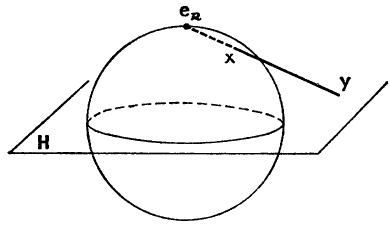
\includegraphics[keepaspectratio]{images/part001_990d2877.jpg}}\\
图 3.

若用 A 表示 \(\{e_{n}\}\) 在 \(S_{n-1}\) 中的补集，这些公式表明我们就这样定义了 A 到超平面 H 上的一个同胚。这个同胚称为 A 到 H 上的球极投影，或（滥用地说）\(S_{n-1}\) 到 H 上的球极投影；\(e_{n}\) 是投影的顶点，H 是投影超平面。更一般地，若 \(H'\) 是过 o 的任一超平面（\(B_{n}\) 的一个直径超平面），且 a 是 \(S_{n-1}\) 与过 o 而垂直于 \(H'\) 的直线的交点之一，我们就可以同样地定义以 a 为顶点、以 \(H'\) 为投影超平面的球极投影；在任何情形下，这个投影都可以通过一个把 \(H'\) 变成 H、把 a 变成 \(e_{n}\) 的正交变换化归为前一个投影。

命题 4. 若 \(n > 1\) ，欧氏球面 \(S_{n-1}\) 同胚于添加一个“无穷远点”而紧化的空间 \(\mathbf{R}^{n-1}\)（第 I 章，§ 9，第 8 小节，定理 4）。

因为球极投影定义了 \(S_{n-1}\) 中一点的补集到 \(R^{n}\) 的一个超平面上的同胚，而这个超平面同胚于 \(R^{n-1}\)。

推论 1. 球面 \(S_{n}\) 同胚于把球 \(B_{n}\) 中球面 \(S_{n-1}\) 的所有点等同起来所得到的商空间。

球 \(B_{n}\) 是正则空间（第 I 章，§ 8，第 4 小节）；因此 \(B_{n}\) 的商空间 F——把 \(S_{n-1}\) 的所有点等同起来而得到的——是豪斯多夫的（第 I 章，§ 8，第 6 小节，命题 15）。由于 \(B_{n}\) 是紧的，F 也是紧的，从而由亚历山德罗夫定理（第 I 章，§ 9，第 8 小节，定理 4），F 同胚于添加一个无穷远点而紧化的 n 维开球。因此结论由命题 2 与命题 4 得出。

推论 2. 圆周 \(\mathbf{S}_1\) 同胚于环面 \(\mathbf{T}\)。

在第 VIII 章，§ 2，第 1 小节中，我们将作为一个更精确的定理的推论重新得到这个结果。

命题 5. 若 \(n > 1\) ，欧氏球面 \(\mathbf{S}_{n-1}\) 是连通的且局部连通的，并且它的每个点都有一个同胚于 \(\mathbf{R}^{n-1}\) 的开邻域。

\(S_{n-1}\) 中一点的补集是连通的稠密集，因此（第 I 章，§ 11，第 1 小节，命题 1）\(S_{n-1}\) 是连通的。要看出每个点都有一个同胚于 \(R^{n-1}\) 的邻域，只需从一个异于该给定点的顶点作球极投影即可。

由这个命题以及第 3 小节的命题 3 推出，\(\mathbf{R}_n^*\) 作为两个连通空间的乘积是连通的（第 I 章，§ 11，第 4 小节，命题 8；参见 § 1，习题 10）。

\(S_{n-1}\) 与 \(B_{n}\) 的一个直径超平面所决定的闭（相应地，开）半空间的交，称为 \(S_{n-1}\) 的闭（相应地，开）半球面。通过到该直径超平面上的球极投影，不含投影顶点的闭（相应地，开）半球面被映成一个 n - 1 维的闭（相应地，开）球，从而同胚于它。

当 n = 2 时，我们说“半圆周”而不说“半球面”。

\section{实射影空间}

在本节中我们需要不断地引用有关商空间的概念和结果（第 I 章，§ 3），特别是下面两条性质，为方便起见我们把它们陈述为引理：

设 E 是拓扑空间，R 是 E 上的一个等价关系，A 是 E 的一个子集，\(R_{A}\) 是 R 在 A 上诱导的等价关系，f 是 E 到 E/R 上的典范映射。那么：

引理 1. 若 A 中每个关于 \(R_{A}\) 饱和的开（相应地，闭）集，都是 E 中关于 R 饱和的开（相应地，闭）集在 A 上的迹，则商空间 \(A/R_{A}\) 同胚于 E/R 的子空间 \(f(A)\)。特别地，当 A 在 E 中是开的或闭的且关于 R 饱和时，情形就是如此。

这由第 I 章，§ 3，第 6 小节，命题 10 得出。

引理 2. 若存在连续映射 \(g\) ——\(\mathbf{E}\) 到 \(\mathbf{A}\) 上的——，使得对一切 \(x \in \mathbf{E}\) ，\(g(x)\) 属于 \(x\) 的等价类，则商空间 \(\mathrm{A} / \mathrm{R}_{\mathbf{A}}\) 同胚于 \(\mathbf{E} / \mathbf{R}\)。

这就是第 I 章，§ 3，第 6 小节，命题 10 的推论 2。

\subsection{实射影空间的拓扑}

我们回忆代数中的下述定义：给定一个除环或域 \(\mathbf{K}\) ，把过 \(o\) 的直线（即一维向量子空间）——左向量空间 \(\mathbf{K}_s^{n+1}\) （\(\mathbf{K}\) 上的）中的——所成的集，称为 \(n\) 维左射影空间（\(\mathbf{K}\) 上的），记作 \(\mathbf{P}_n(\mathbf{K})\)。

若把 \(K_{s}^{n+1}\) 中过 o 的每条直线对应于同一条去掉原点的直线，我们就得到 \(\mathbf{P}_{n}(\mathbf{K})\) 到 \(K_{n+1}^{*}\) （\(\{o\}\) 在 \(K_{s}^{n+1}\) 中的补集）关于下述等价关系 \(\Delta_{n}(\mathbf{K})\) 的商上的一个双射，这个等价关系定义在 \(K_{n+1}^{*}\) 的向量 x 与 y 之间：“存在 \(t \in K\) 使得 \(t \neq o\) 且 y = tx”。在下文中我们将把 \(P_{n}(\mathbf{K})\) 与这个商集等同起来。在射影空间的理论中，我们取 N 的区间 \([o, n]\) 作为 \(K_{n+1}^{*}\) 的点的坐标的指标集。坐标 \(x_{i}\) （ \(o \leqslant i \leqslant n\) ）——\(K_{n+1}^{*}\) 中典范象为 \(x \in P_{n}(\mathbf{K})\) 的任何一点的坐标——组成所谓的点 x 的齐次坐标系。

对每个整数 \(p\) （使 \(-1 \leqslant p \leqslant n\) 的），\(\mathbf{P}_n(\mathbf{K})\) 中一个 \(p + 1\) 维向量子空间（\(\mathrm{K}_s^{n+1}\) 的，去掉原点）的典范象称为 \(p\) 维射影线性簇。\(p\) 个点（\(\mathbf{P}_n(\mathbf{K})\) 中的）组成的一个系称为自由的，如果它由 \(p\) 个点——\(\mathrm{K}_{n+1}^*\) 的、在向量空间 \(\mathrm{K}_s^{n+1}\) 中构成自由系的——的典范象组成。\(\mathbf{P}_n(\mathbf{K})\) 中由 \(p + 1\) 个点的自由系生成的射影线性簇（即包含这 \(p + 1\) 个点的最小射影线性簇）是 \(p\) 维的。

当 K 是域 R 时，相应的射影空间可以赋以拓扑，我们将研究的就是这些空间。

定义 1. 射影空间 \(\mathbf{P}_n(\mathbf{R})\) ——赋以 \(\mathbf{R}_{n+1}^*\) 的拓扑关于等价关系 \(\Delta_n(\mathbf{R})\) 的商拓扑——，称为 \(n\) 维实射影空间。

射影空间 \(\mathbf{P}_{1}(\mathbf{R})\) 称为实射影直线，\(\mathbf{P}_{2}(\mathbf{R})\) 称为实射影平面。

每当没有混淆的危险时，我们将用 \(P_{n}\) 与 \(\Delta_{n}\) 代替 \(\mathbf{P}_{n}(\mathbf{R})\) 与 \(\Delta_{n}(\mathbf{R})\)。

命题 1. 射影空间 \(P_{n}\) 是豪斯多夫的。

我们首先证明关系 \(\Delta_{n}\) 是开的（第 I 章，§ 5，第 2 小节）。设 A 是 \(\mathbf{R}_{n+1}^{*}\) 中的开集；要使 A 关于 \(\Delta_{n}\) 饱和，须取与 A 位似的诸集 \(t\mathbf{A}\) 的并，这里 \(t\) 取遍 \(\neq 0\) 的实数的集；由于这些集中每一个都是开的，它们的并也是开的。

由第 I 章，§ 8，第 3 小节的命题 8，只要证明 \(\mathbf{R}_{n+1}^{*}\times\mathbf{R}_{n+1}^{*}\) 的由关系 \(\Delta_{n}\) 定义的子集 M 是闭的，命题即得证明。设 \((x,y)\) 是 \(\mathbf{R}_{n+1}^{*}\times\mathbf{R}_{n+1}^{*}\) 中属于 M 的闭包的一点。若 \(x=(x_{i})\) ，则有指标 \(i\) 使 \(x_{i}\neq0\) ；因此存在 \((x,y)\) 的邻域 V，使得对每一点 \((x^{\prime},y^{\prime})\in\mathbf{M}\cap\mathbf{V}\) ，第 \(i\) 个坐标 \(x_{i}^{\prime}\) （\(x^{\prime}\) 的）不是 o。当 \((x^{\prime},y^{\prime})\) 保持属于 M 而趋于 \((x,y)\) 时，\(y_{i}^{\prime}x_{i}^{\prime-1}\) 趋于 \(t=y_{i}x_{i}^{-1}\) ；由于 \(y^{\prime}=(y_{i}^{\prime}x_{i}^{\prime-1})x^{\prime}\) ，取极限便见 \(y=tx\) ，这表明 \((x,y)\in\mathbf{M}\) 。

命题 2. 射影空间 \(\mathbf{P}_{n}\) 是紧的且连通的，并且同胚于球面 \(\mathbf{S}_{n}\) 关于 \(\Delta_{n}\) 在该球面上诱导的等价关系的商。

令 \(\Delta_n'\) 是 \(\mathbf{S}_n\) 上由 \(\Delta_n\) 诱导的等价关系（\(\Delta_n'\) 的等价类是 \(\mathbf{S}_n\) 的对径点对）。映射 \(x \to x/||x||\) （\(\mathbf{R}_{n+1}^*\) 到 \(\mathbf{S}_n\) 上的）是连续的，因此（引理 2）\(\mathbf{P}_n\) 同胚于 \(\mathbf{S}_n/\Delta_n'\)。由于 \(\mathbf{S}_n\) 是紧的且连通的，\(\mathbf{S}_n\) 的每个豪斯多夫商空间也是紧的且连通的（第 I 章，§ 9，第 4 小节，定理 2 的推论 1；§ 11，第 3 小节，命题 7）。

命题 3. 若 \(n \geqslant 0\) ，射影空间 \(\mathbf{P}_n\) 同胚于把球 \(\mathbf{B}_n\) 中 \(\mathbf{S}_{n-1}\) 的每个点与其对径点等同起来所得到的商空间。

设 H 是 \(S_{n}\) 的由 \(x_{0} \leqslant 0\) 定义的闭半球面。\(P_{n}\) ——它同胚于 \(S_{n}\) 关于关系 \(\Delta_{n}^{\prime}\) 的商空间——也同胚于 \(S_{n}\) 的子集 H 关于关系 \(\Delta_{n}^{\prime\prime}\) （由 \(\Delta_{n}^{\prime}\) 在 H 上诱导的）的商。由于 \(\Delta_{n}^{\prime}\) 的每个等价类都至少与 H 交于一点，因此（引理 1）只需验证：关于 \(\Delta_{n}^{\prime}\) 把 U （H 的开子集，关于 \(\Delta_{n}^{\prime\prime}\) 饱和）加以饱和化，就得到 V ——\(S_{n}\) 的一个开子集。现在，若 \(a = (a_{i}) \in U\) 且 \(a_{0} < 0\) ，则存在邻域 W （a 的，在 \(S_{n}\) 中的）含于 U，而 W 与 \(-W\) 的并是 a 的一个关于 \(\Delta_{n}^{\prime}\) 饱和且含于 V 的邻域。反之若 \(a_{0} = 0\) ，我们有 \(- a \in U\) ，且存在 r \textgreater{} o，使得点 \(x \in H\) ——满足关系 \(||x-a||<r, ||x+a||<r\) 之一的——所成的集合含于 U；点 \(x\in S_{n}\) ——满足这两个关系之一的——所成的集合就是 a 的那个关于 \(\Delta_{n}^{\prime}\) 饱和且含于 V 的邻域。

注意，商空间 \(H/\Delta_{n}^{\prime\prime}\) 是在 H 中把 \(S_{n-1}\) （即 H 与超平面 \(x_{0}=0\) 的交）的每个点与其相反点等同起来而得到的。要完成证明，只需注意以 \(e_{0}\) 为顶点的球极投影（§ 2，第 4 小节）是 H 到 \(B_{n}\) 上的同胚，且保持 \(S_{n-1}\) 的点不变。

\subsection{射影线性簇}

每个单射线性映射 \(f\) ——\(\mathbf{R}^{n+1}\) 到 \(\mathbf{R}^{m+1}\) 中的（ \(m \geqslant n\) ）——通过限制到 \(\mathbf{R}_{n+1}^*\) 再关于关系 \(\Delta_n\) 与 \(\Delta_m\) 取商（《集合论》，R，§ 5，第 8 小节），定义了一个单射映射 \(g\) ——\(\mathbf{P}_n\) 到 \(\mathbf{P}_m\) 中的——，称为射影线性映射。若 \(\varphi\) （相应地，\(\psi\)）是 \(\mathbf{R}_{n+1}^*\) 到 \(\mathbf{P}_n\) 上（相应地，\(\mathbf{R}_{m+1}^*\) 到 \(\mathbf{P}_m\) 上）的典范映射，则我们有 \(g \circ \varphi = \psi \circ f\) ，这表明 \(g\) 在 \(\mathbf{P}_n\) 上连续（第 I 章，§ 3，第 4 小节，命题 6 的推论）。特别地，\(\mathbf{P}_n\) 的每个射影线性变换（即 \(\mathbf{P}_n\) 到其自身的射影线性映射）是 \(\mathbf{P}_n\) 到其自身的一个同胚。

我们还回忆，若 V 与 \(V'\) 是两个 p 维射影线性簇（\(P_{n}\) 中的），则存在 \(P_{n}\) 的一个射影线性变换把 V 变换为 \(V'\)。特别地，若 \(p \geqslant 0\) ，则存在把 V 变换成坐标射影线性簇的射影线性变换，也就是说，变换成坐标簇 \(W'\) （\(p + 1\) 维的，\(R^{n+1}\) 的，去掉点 o 的）的典范象。若把 \(W'\) 与 \(R_{p+1}^{*}\) 等同，\(\Delta_{n}\) 在 \(W'\) 上诱导的关系正是 \(\Delta_{p}\) ；由于 \(W'\) 是闭的且关于 \(\Delta_{n}\) 饱和，引理 1 表明 \(V'\) 同胚于 \(P_{p}\) 且在 \(P_{n}\) 中是闭的；此外，若 p \textless{} n，它的补集在 \(P_{n}\) 中稠密（§ 1，第 4 小节，命题 3 的推论）。因此：

命题 4. 射影空间 \(P_{n}\) 中每个 p 维射影线性簇在 \(P_{n}\) 中是闭的，且同胚于 \(P_{p}\)；若 p \textless{} n，其补集在 \(P_{n}\) 中稠密。

这个结果是在任意除环上的射影空间中把一维与二维射影线性簇称为射影直线与射影平面这些名称的由来。我们还回忆，\(P_{n}\) 中 n - 1 维的射影线性簇称为射影超平面；每个射影超平面等同于齐次坐标满足形如 \(\sum_{i=0}^{n}a_{i}x_{i}=0\) 的关系（其中诸 \(a_{i}\) 不全为零）的点所成的集（超平面的“方程”）。

\pandocbounded{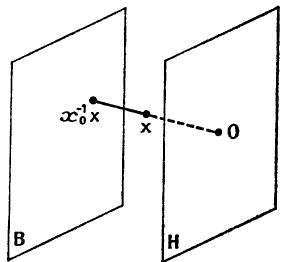
\includegraphics[keepaspectratio]{images/part001_d597a17f.jpg}}\\
图 4.

命题 5. 在射影空间 \(\mathbf{P}_n\) （ \(n \geqslant 0\)）中，射影超平面 H 的补集同胚于 \(\mathbf{R}^n\)。

作一个射影线性变换，我们可以假设 H 是方程为 \(x_{0}=0\) 的超平面。集 A ——由点 \(\boldsymbol{x}=(x_{i})\) （\(R_{n+1}^{*}\) 的，满足 \(x_{0}\neq0\) 的）组成——是开的且关于 \(\Delta_{n}\) 饱和；它的典范象 C （在 \(P_{n}\) 中的）——即 H 在 \(P_{n}\) 中的补集——因此同胚于 A 关于等价关系 \(\Theta\) （由 \(\Delta_{n}\) 在 A 上诱导的）的商（引理 1）。令 B 是方程为 \(x_{0}=1\) 的超平面（\(R^{n+1}\) 中的）。对每一点 \(x\in A\) ，使它对应于点 \(x_{0}^{-1}x\) ，即过 o 与 x 的直线和 B 的交点（图 4）；这样我们定义了 A 到 B 上的连续映射 g，使 \(g(x)\) 是 B 中与 x 模 \(\Theta\) 同余的唯一的点。由此推出 B 同胚于 A/ \(\Theta\) （引理 2），从而同胚于 C；由于 B 同胚于 \(R^{n}\) ，证明完成。

推论. \(P_{n}\) 的每个点都有一个同胚于 \(R^{n}\) 的开邻域。特别地由此推出实射影空间是局部连通的（这也可由第 I 章，§ 11，第 6 小节，命题 12 得出）。

\subsection{实数空间到射影空间中的嵌入}

第 2 小节的命题 5 表明，若在 \(P_{n}\) （ \(n \geqslant 0\)）中给定一个射影超平面 H ，就存在 \(R^{n}\) 到该超平面的补集 \(\complement H\) 上的一个同胚。一旦选定了 H ，用命题 5 中定义的同胚把 \(R^{n}\) 与 \(\complement H\) 等同起来常常是方便的；这时称射影超平面 H 位于“无穷远”，它的点和子集也是如此。通常取 H 为方程为 \(x_{0}=0\) 的“坐标”超平面，于是点 \(z=(z_{i})\) （\(R^{n}\) 的）就与 \(P_{n}\) 中齐次坐标为 \(1, z_{1}, z_{2}, \ldots, z_{n}\) 的点等同。

一旦作了这个等同，在 \(P_{n}\) 中，任何仿射线性簇 V （p 维的，\(R^{n}\) 中的）的闭包是一个 p 维射影线性簇，不含于无穷远超平面中，且等同于由 V 生成的射影线性簇。反之，每个射影线性簇 P （p 维的，不含于无穷远超平面的）在 \(R^{n}\) 上的迹是一个 p 维仿射线性簇，它在 \(P_{n}\) 中的闭包就是 P。

在特例 \(n = 1\) ，无穷远超平面是一个点；由于 \(\mathbf{P}_1\) 是紧的，由亚历山德罗夫定理（第 I 章，§ 9，第 8 小节，定理 4），\(\mathbf{P}_1\) 同胚于空间 \(\tilde{\mathbf{R}}\) ——由局部紧空间 \(\mathbf{R}\) 添加一个点（“无穷远点”）而紧化所得到的——。由 § 2 第 4 小节的命题 4，我们还看出实射影直线 \(\mathbf{P}_1(\mathbf{R})\) 同胚于圆周 \(\mathbf{S}_1\) 以及环面 \(\mathbf{T}\)。

另一方面，若 \(n > 1\) ，\(\mathbf{P}_n(\mathbf{R})\) 不同胚于 \(\mathbf{S}_n\) ，这一点我们以后将会看到（参见习题 4）。

空间 \(\tilde{R}\) 的“无穷远点”记作 \(\infty\) ，不带正负号。重要的是不要把 \(\tilde{R}\) 与第 IV 章，§ 4 中定义的扩充实直线 \(\overline{R}\) 相混淆，后者有两个“无穷远点”；事实上，\(\tilde{R}\) 同胚于 \(\overline{R}\) 的商空间——把两点 \(+\infty\) 与 \(-\infty\) 等同起来所得到的。

\subsection{在实值函数的延拓中的应用}

由于 \(\mathbf{R}\) 可以看作 \(\tilde{\mathbf{R}}\) 的一个子集，每个集 \(\mathbf{E}\) 到 \(\mathbf{R}\) 中的映射（即 \(\mathbf{E}\) 上的每个实值函数）都可以看作 \(\mathbf{E}\) 到 \(\tilde{\mathbf{R}}\) 中的映射；特别地，若 \(\mathbf{E}\) 是拓扑空间 \(\mathbf{F}\) 的子集，且 \(f\) 是 \(\mathbf{E}\) 到 \(\mathbf{R}\) 中的映射，则可能发生这样的情形：在闭包 \(\overline{\mathbf{E}}\) ——\(\mathbf{E}\) 的闭包——的某些点处，\(f(x)\) 趋于极限 \(\infty\) （当 \(x\) 保持属于 \(\mathbf{E}\) 而趋于这些点之一时）；这时我们就可以把函数 \(f\) 连续延拓，在这些点处给它值 \(\infty\)（第 I 章，§ 8，第 5 小节，定理 1）。

特别地考察 E 是 \(R^{n}\) 的子集的情形，这时空间 \(R^{n}\) 本身看作嵌入在射影空间 \(P_{n}\) 中；若假设无穷远超平面是 \(x_{0}=0\) ，定义在 E 上的实值函数 f 就可以等同于映射

\[
(x _ {0}, x _ {1}, x _ {2}, \ldots , x _ {n}) \rightarrow f \left(\frac {x _ {1}}{x _ {0}}, \frac {x _ {2}}{x _ {0}}, \ldots , \frac {x _ {n}}{x _ {0}}\right)
\]

（E 到 \(\tilde{R}\) 中的映射）；由上一段所说的，这个函数可能不仅可以在 E 的闭包中的 \(R^{n}\) 的某些点处延拓，而且可以在 E 的闭包中 \(P_{n}\) 的某些“无穷远点”处延拓。

让我们证明，用这个方法可以得到例如代数中已经定义的一个实变量的有理函数到整个 \(\tilde{\mathbf{R}}\) 上的连续延拓。让我们把 \(\tilde{\mathbf{R}}\) 与 \(\mathbf{P}_1\) 等同起来，每个实数 \(x \in \mathbb{R}\) 等同于齐次坐标为 (1, x) 的点，而点 \(\infty\) 等同于齐次坐标为 (0,1) 的点。设 \(u(x)/v(x)\) 是一个有理函数，\(u\) 与 \(v\) 是次数分别为 \(m\) 与 \(n\) 的两个互素多项式；若例如假设 \(m \leqslant n\) ，并令 \(u_1(x,y) = x^n u(y/x)\) ，\(v_1(x,y) = x^n v(y/x)\) ，则有理函数 \(u/v\) ——在由实数 \(x\) （满足 \(v(x) \neq 0\) 的）组成的集上——可以看作映射 \((x,y) \to (v_1(x,y), u_1(x,y))\) 的限制。换句话说，我们把 \(u/v\) 连续延拓，给它值 \(\infty\) 于那些点 \(x \in \mathbb{R}\) ——使 \(v(x) = 0\) 的——处，并在点 \(\infty\) 处给它值 \(0\) （若 \(m < n\)）、值 \(\infty\) （若 \(m > n\)）、或首项系数之比（若 \(m = n\)）。

特别地，函数 \(1 / x\) 可以延拓到点 \(o\) ，在那里取值 \(\infty\) ，也可延拓到 \(\infty\) ，在那里取值 \(o\) ；这个延拓了的函数显然是 \(\tilde{\mathbf{R}}\) 到其自身的一个同胚。分式线性函数 \((ax + b) / (cx + d)\) （当 \(ad - bc \neq o\) 时）亦然。

同样，若 \(n\) 是 \(> 0\) 的整数，函数 \(x^n\) 可延拓到点 \(\infty\) ，在那里取值 \(\infty\)。

另一方面，两个实变量的有理函数一般不可能连续延拓到空间 \(\mathbf{P}_1 \times \mathbf{P}_1\) 或空间 \(\mathbf{P}_2\)（参见习题 5）。

\subsection{射影线性簇的空间}

给定一个除环 K，集 \(\mathbf{P}_{n,p}(\mathbf{K})\) ——\(p \geqslant 0\) 维射影线性簇（左射影空间 \(\mathbf{P}_{n}(\mathbf{K})\) 的）组成的集——显然与 \(p + 1\) 维向量子空间（左向量空间 \(K_{s}^{n+1}\) 的）组成的集一一对应。令 \(L_{n+1, p+1}(\mathbf{K})\) 表示自由系 \((x_{k})_{1 \leqslant k \leqslant p+1}\) ——\(p + 1\) 个向量（\(K_{s}^{n+1}\) 中的）组成的自由系——所成的集；那么集 \(\mathbf{P}_{n,p}(\mathbf{K})\)

仍然与 \(\mathbf{L}_{n+1,p+1}(\mathbf{K})\) 关于下述等价关系 \(\Delta_{n,p}(\mathbf{K})\) 的商一一对应：“\((\mathbf{x}^{k})\) 与 \((\mathbf{y}^{k})\) 生成同一个 \(p+1\) 维向量子空间（\(K_{s}^{n+1}\) 的）”。在下文中我们将把 \(\mathbf{P}_{n,p}(\mathbf{K})\) 与这个商集等同。另一方面，若把每个自由系 \((\mathbf{x}_{k})\) ——\(p+1\) 个向量（\(K_{s}^{n+1}\) 中的）组成的——对应于矩阵 X ——\(p+1\) 行 \(n+1\) 列的，以 \(x_{k}\) 为第 k 行（ \(1\leqslant k\leqslant p+1\) ）——，我们就得到 \(L_{n+1,p+1}(\mathbf{K})\) 与所有 \(p+1\) 行 \(n+1\) 列、秩为 \(p+1\) 的矩阵组成的集之间的一一对应；我们将把 \(L_{n+1,p+1}(\mathbf{K})\) 与这个矩阵集等同，而两个矩阵 X, Y 之间的关系 \(\Delta_{n,p}(\mathbf{K})\) 就是：“存在 \(p+1\) 阶非奇异方矩阵 T 使得 Y = T.X”。

在下文中我们取 K 为域 R，并在上述记号中省略字母 K。我们可以用一种推广实射影空间拓扑定义的办法来定义 \(P_{n,p}\) 上的拓扑。即，\(L_{n+1, p+1}\) 含于空间 \(M_{p+1, n+1}\) ——以实数为元素的 \(p + 1\) 行 \(n + 1\) 列的一切矩阵组成的空间——；我们给 \(L_{n+1, p+1}\) 赋以这个矩阵空间的拓扑所诱导的拓扑（§ 1，第 6 小节）。

定义 2. 空间 \(\mathbf{P}_{n,p}\) ——拓扑空间 \(\mathbf{L}_{n+1,p+1}\) 关于等价关系 \(\Delta_{n,p}\) 的商——称为 \(p\geqslant0\) 维射影线性簇（在实射影空间 \(\mathbf{P}_{n}\) 中的）的空间。

我们将使用下述记号：给定一个 \(p + 1\) 行 \(n + 1\) 列的矩阵 X，以及任一严格递增序列

\[
\sigma = (i _ {1}, \dots , i _ {p + 1})
\]

的 \(p + 1\) 个指标（区间 \([0, n]\) ，属于 \(\mathbf{N}\) ），我们用 \(X_{\sigma}\) 表示 \(X\) 的由指标为 \(i_1, i_2, \ldots, i_{p+1}\) 的列组成的方子矩阵。我们用 \(\mathbf{A}_{\sigma}\) 表示 \(\mathbf{L}_{n+1, p+1}\) 中由这些矩阵 \(X\) ——使 \(X_{\sigma}\) 非奇异的——组成的子集。由 § 1 第 6 小节的命题 6，\(\mathbf{A}_{\sigma}\) 是 \(\mathbf{M}_{p+1, n+1}\) 中的稠密开集，而且函数 \(X \to X_{\sigma}^{-1}\) 在 \(\mathbf{A}_{\sigma}\) 上连续。

集 \(A_{\sigma}\) 的一个几何解释如下：设 \(E_{\sigma}\) 是 \(R^{n+1}\) 中由典范基的向量 \(e_{i}\) （使 \(i \in \sigma\) 的）生成的向量子空间，设 \(E_{\sigma}'\) 是由 \(e_{i}\) （使 \(i \notin \sigma\) 的）生成的余子空间；那么说矩阵 x 属于 \(A_{\sigma}\) ，意思是其在 \(E_{\sigma}\) 上的投影——它的 \(p + 1\) 行（即 \(x_{k}\)）的投影——构成自由系，或者说，由诸 \(x_{k}\) 生成的向量子空间是 \(E_{\sigma}'\) 的余子空间（或者说它与 \(E_{\sigma}'\) 的交只由 o 组成）。

命题 6. 空间 \(\mathbf{P}_{n,p}\) 是豪斯多夫的。

我们首先证明关系 \(\Delta_{n,p}\) 是开的。若 U 是 \(L_{n+1,p+1}\) 中的开集，要使 U 关于 \(\Delta_{n,p}\) 饱和，须取 U 在映射 \(X \to T \cdot X\) 下的象的并，这里 T 取遍 \(p + 1\) 阶非奇异方矩阵的集；由于这些映射中每一个都是双连续的，所有这些象都是开集，因此它们的并也是开集。

由第 I 章，§ 8，第 3 小节的命题 8，只要证明 \(L_{n+1,p+1} \times L_{n+1,p+1}\) 的由 \(\Delta_{n,p}\) 定义的子集 N 是闭的，证明即告完成。设 \((X,\mathcal{Y})\) 是乘积空间中属于 N 的闭包的一点，设 \(\sigma\) 是使 \(X_{\sigma}\) 非奇异的指标序列：由于 \(A_{\sigma}\) 是开的，存在 \((X,\mathcal{Y})\) 的邻域 V，使得对每对 \((X',\mathcal{Y}') \in \mathrm{N} \cap \mathrm{V}\) ，矩阵 \(X'_{\sigma}\) 都是非奇异的；当 \((X',\mathcal{Y}')\) 保持属于 N 而趋于 \((X,\mathcal{Y})\) 时，矩阵 \(Y'_{\sigma}X_{\sigma}^{\prime -1}\) 就趋于 \(T = Y_{\sigma}X_{\sigma}^{-1}\) ；由于我们有 \(Y' = (Y'_{\sigma}X_{\sigma}^{\prime -1})X'\) ，取极限便见 Y = T.X，证明完成。

命题 7. 空间 \(\mathbf{P}_{n,p}\) 是紧的。

只需证明存在 \(L_{n+1, p+1}\) 的一个紧子空间，它与模 \(\Delta_{n,p}\) 的每个等价类至少交于一点；因为这时 \(P_{n,p}\) 是这个子空间在 \(L_{n+1, p+1}\) 到 \(P_{n,p}\) 上的典范映射下的象，因此是紧的（第 I 章，§ 9，第 4 小节，定理 2）。

令 \(\mathbf{V}_{n+1, p+1}\) 是 \(\mathbf{L}_{n+1, p+1}\) 的这样的子空间：其元素是系 \((\boldsymbol{x}_k)\) ——由 \(p + 1\) 个向量组成的——，这些向量构成它们所生成的向量子空间的欧氏标准正交基，也就是说满足 \((x_h | x_k) = 0\) （每当 \(h \neq k\) ），且 \((x_h | x_h) = 1\) （对 \(1 \leqslant h \leqslant p + 1\) ）。每个 \(p + 1\) 维向量子空间（\(\mathbf{R}^{n+1}\) 的）都有这样一个基，因此模 \(\Delta_{n,p}\) 的每个类都与 \(\mathbf{V}_{n+1, p+1}\) 相交。另一方面，矩阵 \(X = (x_{ij})\) ——\(\mathbf{V}_{n+1, p+1}\) 的——由下述关系定义

\[
\sum_ {j = 0} ^ {n} x _ {i j} ^ {2} = 1 (1 \leqslant i \leqslant p + 1),
\]

\[
\sum_ {j = 0} ^ {n} x _ {i j} x _ {k j} = 0 \quad (i \neq k);
\]

因此它们组成 \(M_{p+1, n+1}\) 中的一个闭集；又由于这些关系蕴含 \(|x_{ij}| \leqslant 1\) （对每对指标 \((i, j)\) ），这个集是有界的，从而是紧的。

命题 8. \(\mathbf{P}_{n,p}\) 是连通的且局部连通的，并且每个点都有一个同胚于 \(\mathbf{R}^{(p+1)(n-p)}\) 的开邻域。

对每个（严格递增的）指标序列 \(\sigma\) ，集 \(\mathbf{A}_{\sigma}\) 在 \(\mathbf{L}_{n+1, p+1}\) 中是开的且关于 \(\Delta_{n,p}\) 饱和；它的典范象

\(C_{\sigma}\) （\(P_{n,p}\) 中的）因此是一个开集，同胚于 \(A_{\sigma}\) 关于等价关系 \(\Theta_{\sigma}\) （在 \(A_{\sigma}\) 上由 \(\Delta_{n,p}\) 诱导的）的商（引理 1）。

令 \(\mathbf{B}_{\sigma}\) 是 \(\mathbf{A}_{\sigma}\) 中由矩阵 \(X\) ——使 \(X_{\sigma}\) 为 \(p + 1\) 阶单位矩阵的——组成的子集；\(X\) 中除 \(X_{\sigma}\) 的元素以外的元素这时是任意的，因此 \(\mathbf{B}_{\sigma}\) 同胚于空间 \(\mathbf{R}^{(p + 1)(n - p)}\) 。对每个矩阵 \(X \in \mathbf{A}_{\sigma}\) ，使它对应于矩阵 \(\Upsilon = X_{\sigma}^{-1}X\) ，它属于 \(\mathbf{B}_{\sigma}\) ；这样我们就定义了连续映射 \(g\) ——\(\mathbf{A}_{\sigma}\) 到 \(\mathbf{B}_{\sigma}\) 上的——，使 \(g(X)\) 是 \(\mathbf{B}_{\sigma}\) 中与 \(X\) 模 \(\Theta_{\sigma}\) 同余的唯一的矩阵。由此推出 \(\mathbf{B}_{\sigma}\) 同胚于 \(\mathbf{A}_{\sigma}/\Theta_{\sigma}\) （引理 2），从而同胚于 \(\mathbf{C}_{\sigma}\) 。

集 \(C_{\sigma}\) 因此是连通的。由于 \(A_{\sigma}\) 在 \(L_{n+1, p+1}\) 中稠密，\(C_{\sigma}\) 在 \(P_{n, p}\) 中稠密，因此 \(P_{n, p}\) 也是连通的（第 I 章，§ 11，第 1 小节，命题 1）。另一方面，\(P_{n, p}\) 的每个点都属于 \(C_{\sigma}\) （对至少一个指标序列 \(\sigma\) ），从而有一个同胚于 \(\mathbf{R}^{(p+1)(n-p)}\) 的开邻域。

矩阵 \(Y=g(X)\) 可以解释如下：为简单起见，设序列 \(\sigma\) 由 \(p+1\) 个指标 n-p, \(n-p+1\) , \(\ldots\) , n 组成，并用 \(a_{ij}\) ( \(1\leqslant i\leqslant p+1\) , \(o\leqslant j\leqslant n-p-1\) ) 表示 y 的前 n-p 列的元素；那么由 x 的行生成的 \(R^{n+1}\) 的向量子空间就是由方程

\[
x _ {j} = \sum_ {i = 1} ^ {p + 1} a _ {i j} x _ {n - p + i - 1} \quad (0 \leqslant j \leqslant n - p - 1).
\]

\subsection{格拉斯曼流形}

若 K 是一个域，X 是 \(\mathrm{L}_{n+1,p+1}(\mathrm{K})\) 的任一矩阵，令 \(c_{\sigma}(X)\) 表示 \(X_{\sigma}\) 的行列式；这样，对 \(\mathrm{L}_{n+1,p+1}(\mathrm{K})\) 的每个矩阵 X 就对应

\[
h = \binom {n + 1} {p + 1}
\]

个行列式，它们不全为零（\(p + 1\) 行——\(X\) 的——的外积的分量）。若把 \(X\) 对应到射影空间 \(\mathbf{P}_{h-1}(\mathbf{K})\) 中齐次坐标为诸 \(c_{\sigma}(X)\) 的点，我们就定义了 \(\mathbf{L}_{n+1,p+1}(\mathbf{K})\) 到 \(\mathbf{P}_{h-1}(\mathbf{K})\) 中的一个映射，它与关系 \(\Delta_{n,p}(\mathbf{K})\) 相容；取商，我们因此得到映射 \(f\) ——\(\mathbf{P}_{n,p}(\mathbf{K})\) 到 \(\mathbf{P}_{h-1}(\mathbf{K})\) 中的——。这个映射的象 \(\mathbf{G}_{n,p}(\mathbf{K})\) （\(\mathbf{P}_{n,p}(\mathbf{K})\) 在该映射下的象）称为指标 \(n\) 、\(p\) 的格拉斯曼流形。我们还回忆映射 \(f\) 是单射的，因为若 \(X\) 是使 \(X_{\sigma}\) 非奇异的矩阵，则矩阵 \(\Upsilon = X_{\sigma}^{-1}X\) ——\(\mathbf{B}_{\sigma}\) 中对应于 \(X\) 模 \(\Delta_{n,p}(\mathbf{K})\) 的类的——就是矩阵 \((d_{ij}/c_{\sigma}(X))\) ( \(1 \leqslant i \leqslant p + 1\) , \(0 \leqslant j \leqslant n\) )，其中 \(d_{ij}\) 表示从 \(X_{\sigma}\) 出发、把 \(X_{\sigma}\) 的第 i 列换成 X 的第 j 列所得矩阵的行列式{[}这蕴含 \(d_{ij}\) 与诸 \(c_{\tau}(X)\) 之一相差一个正负号{]}。

当 \(\mathbf{K}\) 是域 \(\mathbf{R}\) 时，这个映射 \(f\) 显然是连续的。逆映射 \(g\) 也是连续的；因为 \(\mathbf{B}_{\sigma}\) 中的矩阵的元素是它所对应的格拉斯曼流形的点的齐次坐标的有理函数；由于 \(f(\mathbf{B}_{\sigma}) = \mathbf{B}_{\sigma}'\) 是 \(\mathbf{G}_{n,p}\) 中指标为 \(\sigma\) 的齐次坐标不为 \(0\) 的点的集，它是 \(\mathbf{G}_{n,p}\) 中的开集；因此 \(g\) 在 \(\mathbf{B}_{\sigma}'\) 的每一点连续，又由于 \(\mathbf{G}_{n,p}\) 的每一点都属于至少一个集 \(\mathbf{B}_{\sigma}'\) ，\(g\) 在每一点都连续。于是：

命题 9. 格拉斯曼流形 \(\mathbf{G}_{n,p}\) 同胚于空间 \(\mathbf{P}_{n,p}\)。

最后我们回忆，格拉斯曼流形 \(\mathbf{G}_{n,p}(\mathbf{K})\) 与 \(\mathbf{G}_{n,n-p-1}(\mathbf{K})\) 是同一射影空间 \(\mathbf{P}_{h-1}(\mathbf{K})\) 的子集，并且可以通过一个射影线性变换互相变换；由此推出 \(G_{n,p}\) 与 \(G_{n,n-p-1}\) 是同胚的。
